% ===================== Backup =====================
\section*{Backup}

\begin{frame}
  \centering \Huge \textbf{Backup slides}
\end{frame}

% Moved from the main talk (nucleon methods and fit details)
\begin{frame}{Backup: proton two-point function (spectral decomposition)}
  On inserting a complete set of states between the interpolating operators\footnote{Refer: Boussarie, Renaud, et al. ``TMD Handbook.'' arXiv:2304.03302 [hep-ph].}
  \begin{align*}
    C_{\alpha\beta}(t,\mathbf{p})=&\,a^{3}\sum_{n,\sigma}\frac{e^{-E_{n}(\mathbf{p})t}}{2E_{n}(\mathbf{p})}\bra{0}\chi_{\alpha}\ket{n;\mathbf{p},\sigma}\bra{n;\mathbf{p},\sigma}\bar{\chi}_{\beta}\ket{0}\\
    =&\,a^{3}Z(\mathbf{p})\sum_{\sigma}u_{\alpha}(n=0,\mathbf{p},\sigma)\bar{u}_{\beta}(n=0,\mathbf{p},\sigma)\frac{e^{-E_{0}(\mathbf{p})t}}{2E_{0}(\mathbf{p})}+\cdots
  \end{align*}
  Tracing this correlator against a given Dirac structure, often chosen to be $\Gamma^{+}=\frac{1}{2}(1+\gamma_{4})$, leads to
  \begin{align*}
    \boxed{C_{\Gamma^{+}}(t,\mathbf{p})}=\Gamma^{+}_{\beta\alpha}C_{\alpha\beta}(t,\mathbf{p})\xrightarrow{t\rightarrow\infty}\boxed{Ce^{-E_{0}(\mathbf{p})t}}
  \end{align*}
  where $C$ is a time-independent constant.
\end{frame}

% Slide 12. Diagram: Can et al., LNP 889 (2015), Fig. 3.8,
% printed p. 84 / PDF p. 97 of the local Lin--Meyer reference.
% Vector crop in PDF points: 266 56 373 149. Labels below are added in LaTeX.
\begin{frame}{Backup: nucleon three-point function}
  \begin{columns}[c]
    \begin{column}{0.56\textwidth}
      \begin{itemize}
        \item The source $\bar\chi$ creates a nucleon at $0$; the sink $\chi$ annihilates it at $t$. Insert $\mathcal O_\Gamma=\bar q\,\Gamma\,q$ at $0<\tau<t$.
        \item The three lines are quark propagators $S=\mathcal M^{-1}$ ($u,u,d$). In a \textbf{connected contraction}, the insertion probes one line.
        \item \textbf{Sequential source:} one extra inversion from the sink gives the propagator to every insertion point.
        \item Disconnected insertions form a separate quark loop. They cancel in $u-d$ for $m_u=m_d$.
      \end{itemize}
    \end{column}
    \begin{column}{0.42\textwidth}
      \centering
      \begin{tikzpicture}
        \node[inner sep=0] (image) {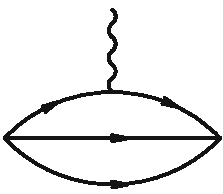
\includegraphics[width=0.62\linewidth]{nucleon_3pt_LinMeyer_fig3_8.pdf}};
        \node[font=\scriptsize, anchor=south, align=center] at (image.north)
          {wavy line: operator insertion\\$\mathcal O_\Gamma(\vect x_1,\tau)=\bar q\,\Gamma\,q$};
        \node[font=\scriptsize, anchor=east, align=center] at ($(image.south west)!0.29!(image.north west)$)
          {source\\$0$};
        \node[font=\scriptsize, anchor=west, align=center] at ($(image.south east)!0.29!(image.north east)$)
          {sink\\$t$};
        \node[font=\scriptsize, anchor=west] at ($(image.south west)!0.60!(image.north east)$)
          {$\tau$};
        \node[font=\scriptsize, anchor=north] at ($(image.south west)!0.22!(image.south east)$)
          {momentum $\vect p$};
        \node[font=\scriptsize, anchor=north] at ($(image.south west)!0.78!(image.south east)$)
          {momentum $\vect p$};
      \end{tikzpicture}\\[3mm]
      \figsrc{K.~U.~Can et al., ``Hadron Structure on the Lattice,''\\
        in Lin \& Meyer (eds.), 2015, Fig.~3.8, p.~84.}
    \end{column}
  \end{columns}
  \vspace{1mm}
  \[
    \begin{aligned}
      G_\Gamma(t,\tau;\vect p)={}&a^6\!\sum_{\vect x_2,\vect x_1}
      e^{-i\vect p\cdot\vect x_2}
      \,\Gamma^{\rm 3pt}_{\beta\alpha}\\[-1mm]
      &\times\big\langle\chi_\alpha(\vect x_2,t)\,
      \mathcal O_\Gamma(\vect x_1,\tau)\,\bar\chi_\beta(\vect 0,0)\big\rangle .
    \end{aligned}
  \]
  \centering
  {\small $\Gamma$: Dirac matrix in the operator;\quad
    $\Gamma^{\rm 3pt}$: nucleon spin projector (like $\Gamma^+$ in the two-point function).\\
    Source and sink have the same momentum $\vect p$.}
\end{frame}

% Slide 13. Normalization follows thesis Eqs. c3pt_ground and ratio_forward, specialized to p'=p.
\begin{frame}{Backup: extracting the nucleon matrix element}
  For the operator $\mathcal O_\Gamma=\bar q\,\Gamma\,q$ with the same momentum $\vect p$ at source and sink, $E=E(\vect p)$ and $K(p)=-i{\not\!p}+m=\sum_s u\bar u$, the ratio of the ground-state terms of $G_\Gamma$ and $C_{\Gamma^+}$ removes the unknown overlap $|Z|$ and the time dependence:
  \[
    R(t,\tau)=\frac{G_\Gamma(t,\tau;\vect p)}{C_{\Gamma^+}(t,\vect p)}
    \simeq
    \frac{\dfrac{|Z(\vect p)|}{4E^2}\,e^{-Et}\,\Tr\!\left[\Gamma^{\rm 3pt}K(p)\,\mathcal J\,K(p)\right]}
         {|Z(\vect p)|\,\dfrac{E+m}{E}\,e^{-Et}}
    =\frac{\Tr[\Gamma^{\rm 3pt}K(p)\,\mathcal J\,K(p)]}{4E(E+m)}
  \]
  {\small $\mathcal O_\Gamma$: the operator;\quad
    $\mathcal J$: Dirac structure of its nucleon matrix element,
    $\langle N(\vect p,s')|\mathcal O_\Gamma|N(\vect p,s)\rangle=\bar u(\vect p,s')\,\mathcal J\,u(\vect p,s)$ (the quantity we extract);\quad
    $\Gamma^{\rm 3pt}$: nucleon spin projector.}
  \begin{itemize}
    \item Ground-state isolation needs $\Delta E\,\tau\gg1$ and $\Delta E\,(t-\tau)\gg1$.
      The \textbf{plateau in $\tau$} then gives the projected matrix element.
      Here $\Gamma^+=\tfrac12(1+\gamma_4)$ and $p_4=iE$.
    \item Larger source--sink separation suppresses excited states, but increases
      statistical noise; plateau stability must be checked.
  \end{itemize}
  \figsrc{Can et al., in Lin \& Meyer (eds.), 2015, Sec.~3.3; thesis lattice methodology.}
\end{frame}

% Fitting methodology 27/32
\begin{frame}{Backup: full Jackknife covariance and correlated fitting}
\[
\bar y_i=\frac1{N_{\rm JK}}\sum_{k=1}^{N_{\rm JK}}y_i^{(k)},\qquad
C_{ij}=\frac{N_{\rm JK}-1}{N_{\rm JK}}\sum_{k=1}^{N_{\rm JK}}
(y_i^{(k)}-\bar y_i)(y_j^{(k)}-\bar y_j).
\]
\[
\boxed{\chi^2(\mathbf p)=\sum_{i,j}[\bar y_i-F_i(\mathbf p)]C^{-1}_{ij}[\bar y_j-F_j(\mathbf p)]}
\]
\begin{itemize}
\item Stack points from all retained spatial coordinates, staple extents, and all three amplitudes.
\item The same gauge configurations create correlations both between coordinates and between amplitude components.
\item Retain the full covariance rather than treating those measurements as independent.
\item Use \texttt{lsqfit} for nonlinear fitting and \texttt{gvar} for correlated Gaussian quantities.
\end{itemize}
\end{frame}

% Moved from the main talk (nucleon two-point function)
\begin{frame}{Backup: nucleon two-point function in terms of propagators}
  After integrating out the quark fields in the path integral formulation, this correlator is expressed in terms of products of the inverse of the Dirac operator
  {\small
  \begin{align*}
    C_{\alpha\beta}(t,\mathbf{p})=&-a^3\sum_{\mathbf{x}}e^{-i\mathbf{p}\cdot\mathbf{x}}\epsilon^{ijk}\epsilon^{i'j'k'}[C^{-1}\gamma_{5}]_{\alpha'\alpha''}[\gamma_{5}C]_{\beta'\beta''}\\
    &\times\left\langle[\mathcal{M}^{-1}_{d}]^{ki'}_{\alpha''\beta'}\left\{[\mathcal{M}^{-1}_{u}]^{jj'}_{\alpha'\beta''}[\mathcal{M}^{-1}_{u}]^{ik'}_{\alpha\beta}-[\mathcal{M}^{-1}_{u}]^{ij'}_{\alpha\beta''}[\mathcal{M}^{-1}_{d}]^{ik'}_{\alpha'\beta}\right\}\right\rangle
  \end{align*}}
\end{frame}

% Moved from main talk (gauge link and process dependence)
\begin{frame}{Backup: why it is not zero, the gauge link}
  \begin{itemize}
    \item Collins (1993): time reversal forces $f_{1T}^\perp=0$ \quad (``naively T-odd'').
    \item Brodsky--Hwang--Schmidt (2002): final-state interactions give a nonzero asymmetry.
    \item Collins (2002): a gauge-invariant TMD needs a \textbf{Wilson line}. Its path depends on the process, and T-reversal swaps the two paths:
  \end{itemize}
  \[ f_{1T}^{\perp}(x,\vprp{k}^2)\Big|_{\text{SIDIS}} = - f_{1T}^{\perp}(x,\vprp{k}^2)\Big|_{\text{DY}} \]
  \centering
  \begin{tikzpicture}[scale=0.8, q/.style={circle, fill=black, inner sep=1.5pt}]
    \begin{scope}[shift={(0,0)}]
      \node[q, label=left:{$0$}] at (0,0) {};
      \node[q, label=left:{$\bvec$}] at (0,1.6) {};
      \draw[very thick, -latex] (0,0) -- (1.9,0);
      \draw[very thick] (1.9,0) -- (3.6,0);
      \draw[very thick, dashed] (3.6,0) -- (3.6,1.6);
      \draw[very thick, -latex] (3.6,1.6) -- (1.6,1.6);
      \draw[very thick] (1.6,1.6) -- (0,1.6);
      \node[right] at (3.65,0.8) {\small $+\infty\,\nminus$};
      \node at (1.8,-0.6) {\small (a) SIDIS: future-pointing};
    \end{scope}
    \begin{scope}[shift={(10.2,0)}]
      \node[q, label=right:{$0$}] at (0,0) {};
      \node[q, label=right:{$\bvec$}] at (0,1.6) {};
      \draw[very thick, -latex] (0,0) -- (-1.9,0);
      \draw[very thick] (-1.9,0) -- (-3.6,0);
      \draw[very thick, dashed] (-3.6,0) -- (-3.6,1.6);
      \draw[very thick, -latex] (-3.6,1.6) -- (-1.6,1.6);
      \draw[very thick] (-1.6,1.6) -- (0,1.6);
      \node[left] at (-3.65,0.8) {\small $-\infty\,\nminus$};
      \node at (-1.8,-0.6) {\small (b) Drell--Yan: past-pointing};
    \end{scope}
  \end{tikzpicture}
  \keymsg{We put this \textbf{staple-shaped link} on the lattice.}
\end{frame}

% Amplitude slices P_L=-2
\begin{frame}{Backup: amplitudes at $P_L=-2$ ($\zetahat=0.294367$), $\eta|v|/a=8$}
  \centering
  \begin{tabular}{cc}
    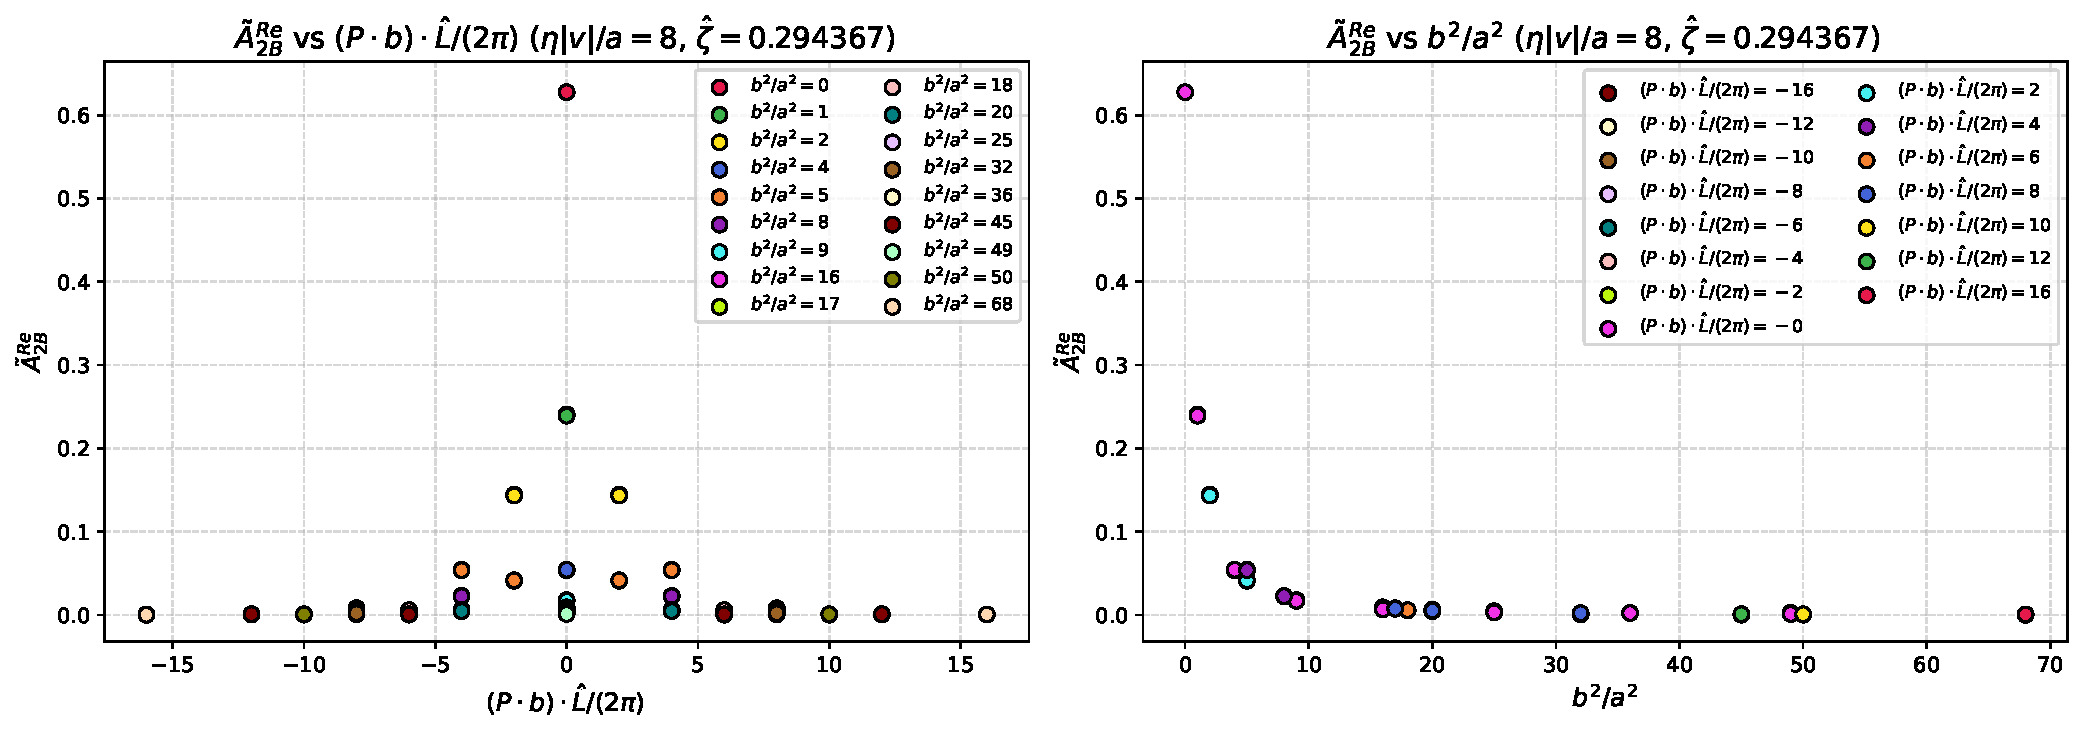
\includegraphics[height=0.38\textheight, trim=0 0 500 0, clip]{ReA2B_Pb_bsq_eta8_PL-2_2D.pdf} &
    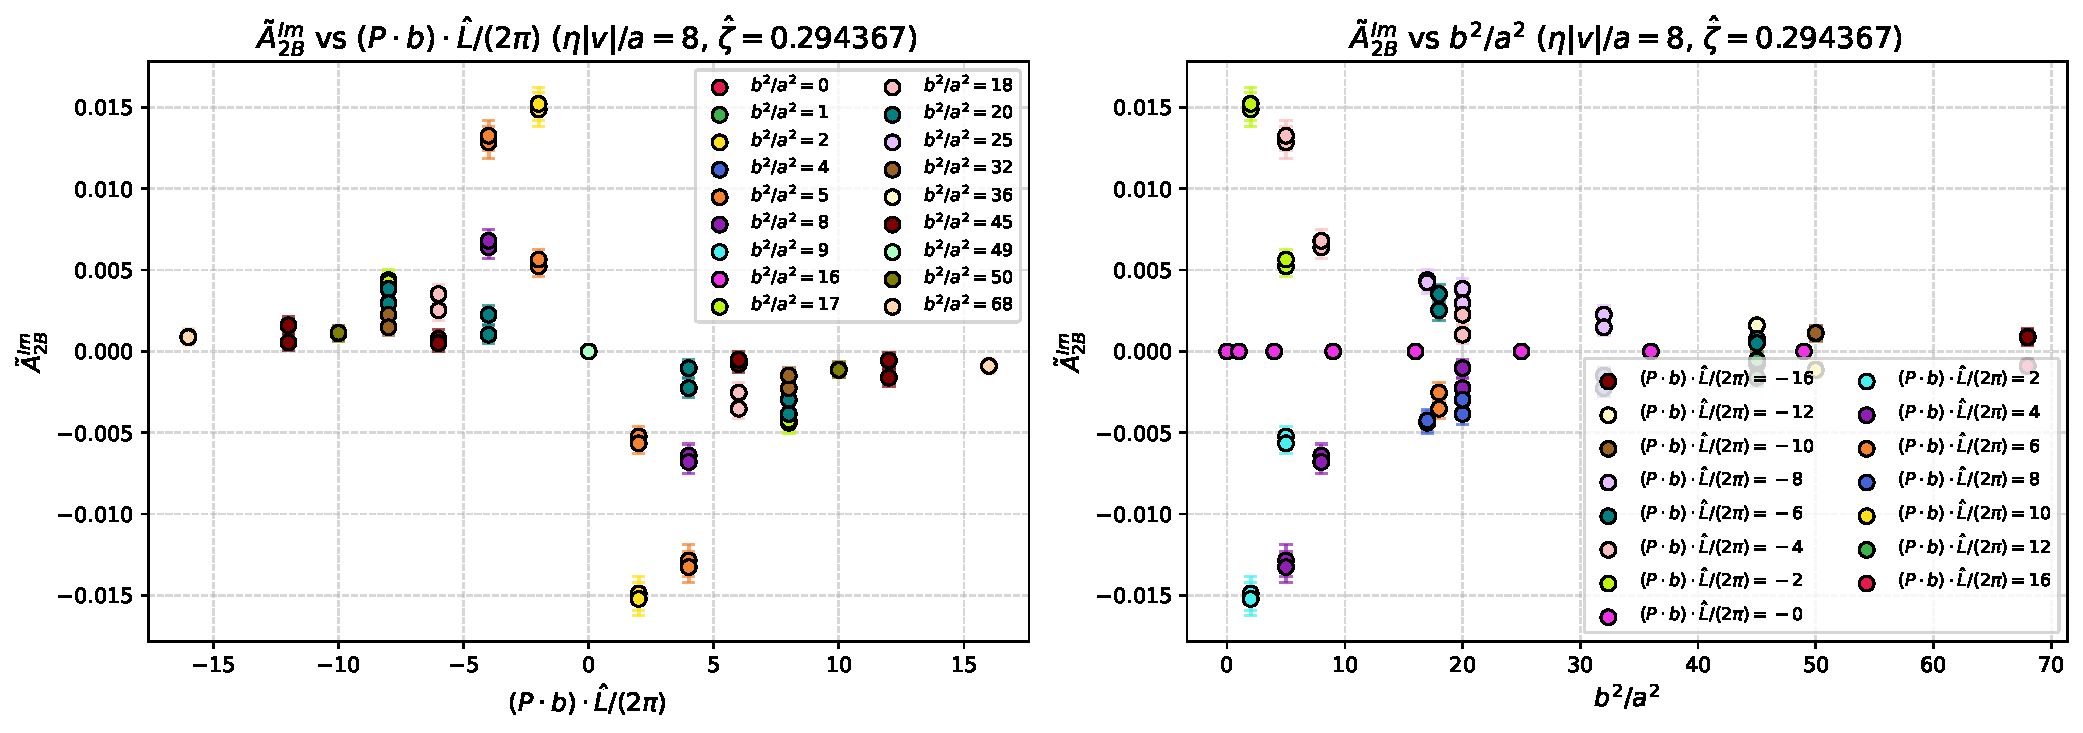
\includegraphics[height=0.38\textheight, trim=0 0 500 0, clip]{ImA2B_Pb_bsq_eta8_PL-2_2D.pdf} \\
    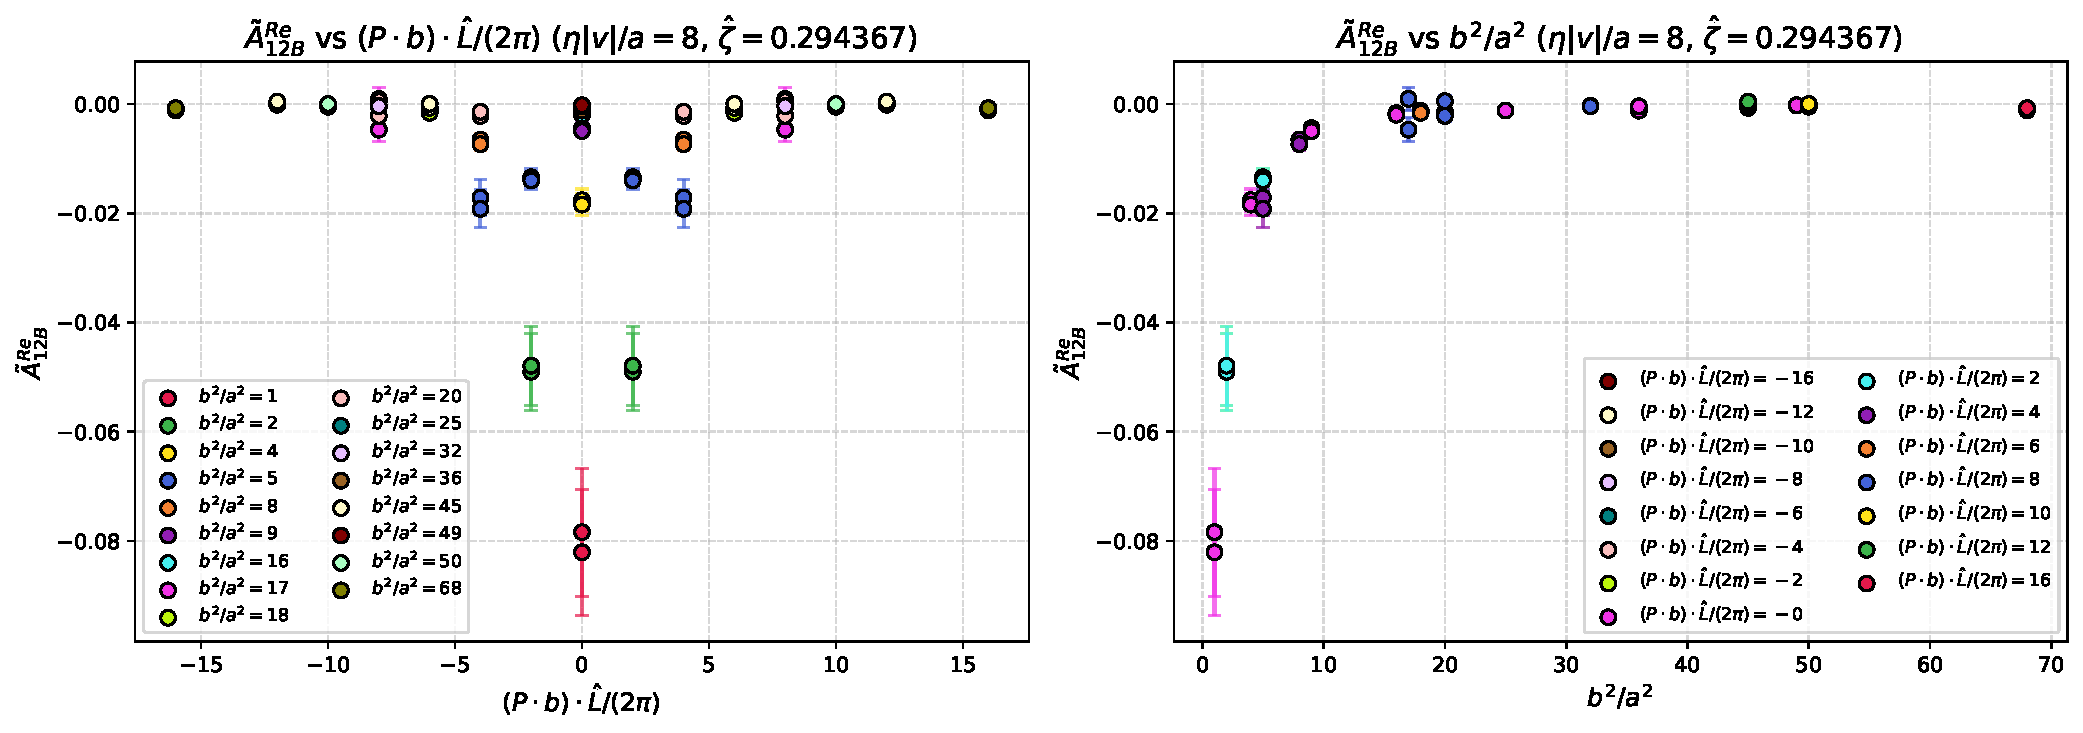
\includegraphics[height=0.38\textheight, trim=0 0 500 0, clip]{ReA12B_Pb_bsq_eta8_PL-2_2D.pdf} &
    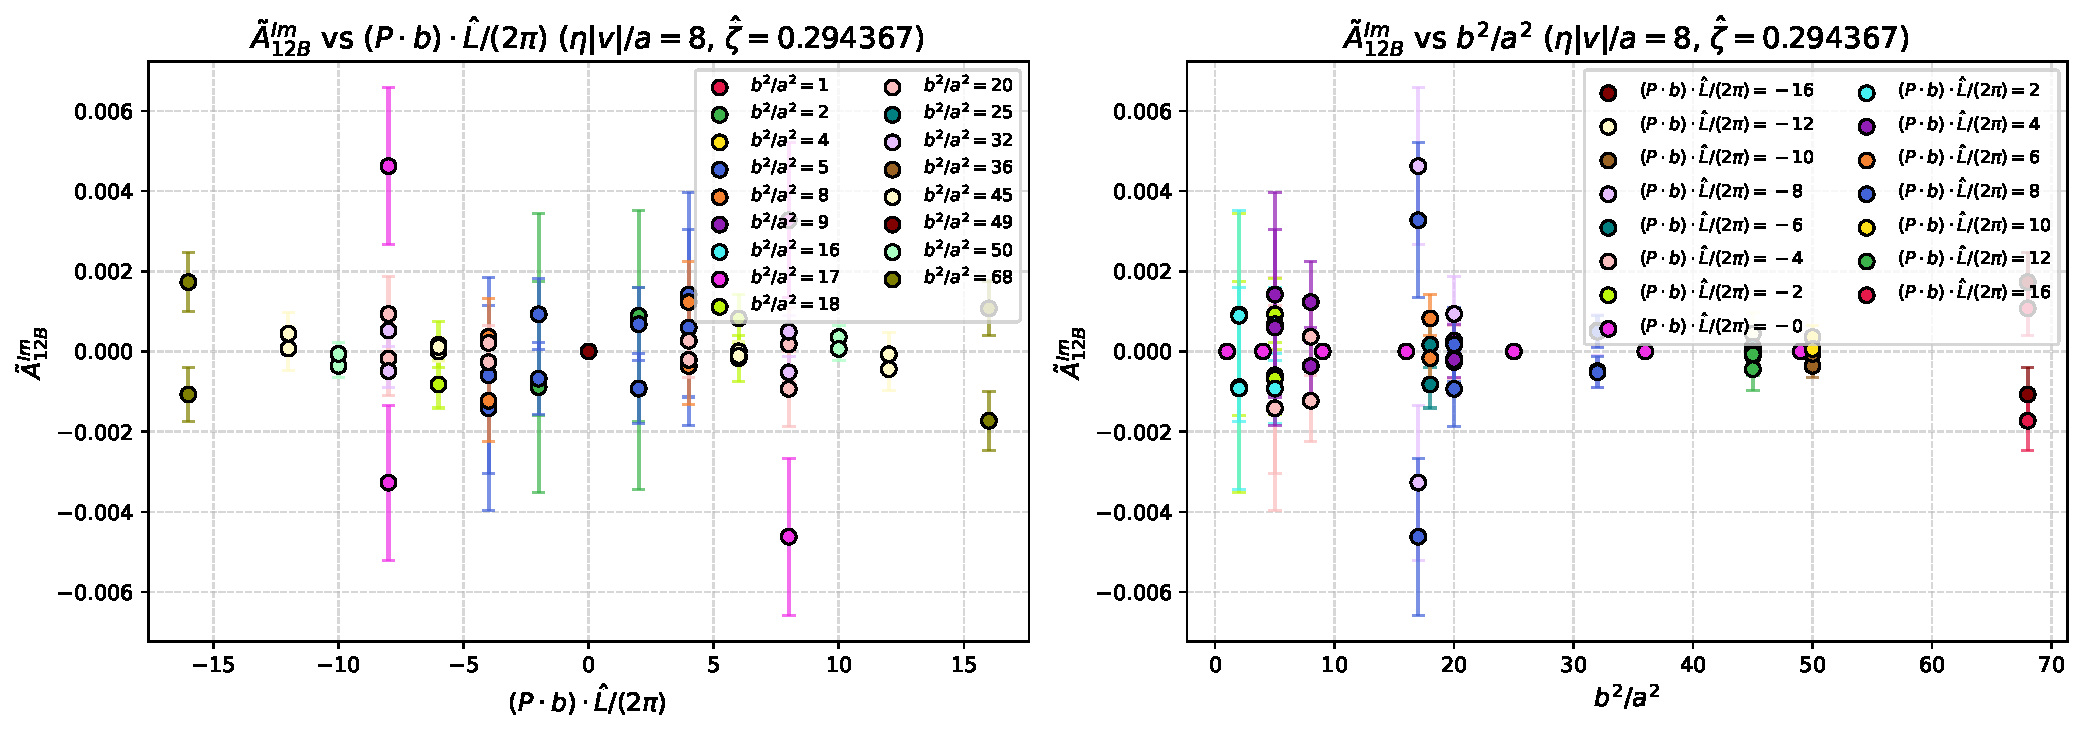
\includegraphics[height=0.38\textheight, trim=0 0 500 0, clip]{ImA12B_Pb_bsq_eta8_PL-2_2D.pdf}
  \end{tabular}
\end{frame}

% Amplitude slices P_L=-3
\begin{frame}{Backup: amplitudes at $P_L=-3$ ($\zetahat=0.539684$), $\eta|v|/a=8$}
  \centering
  \begin{tabular}{cc}
    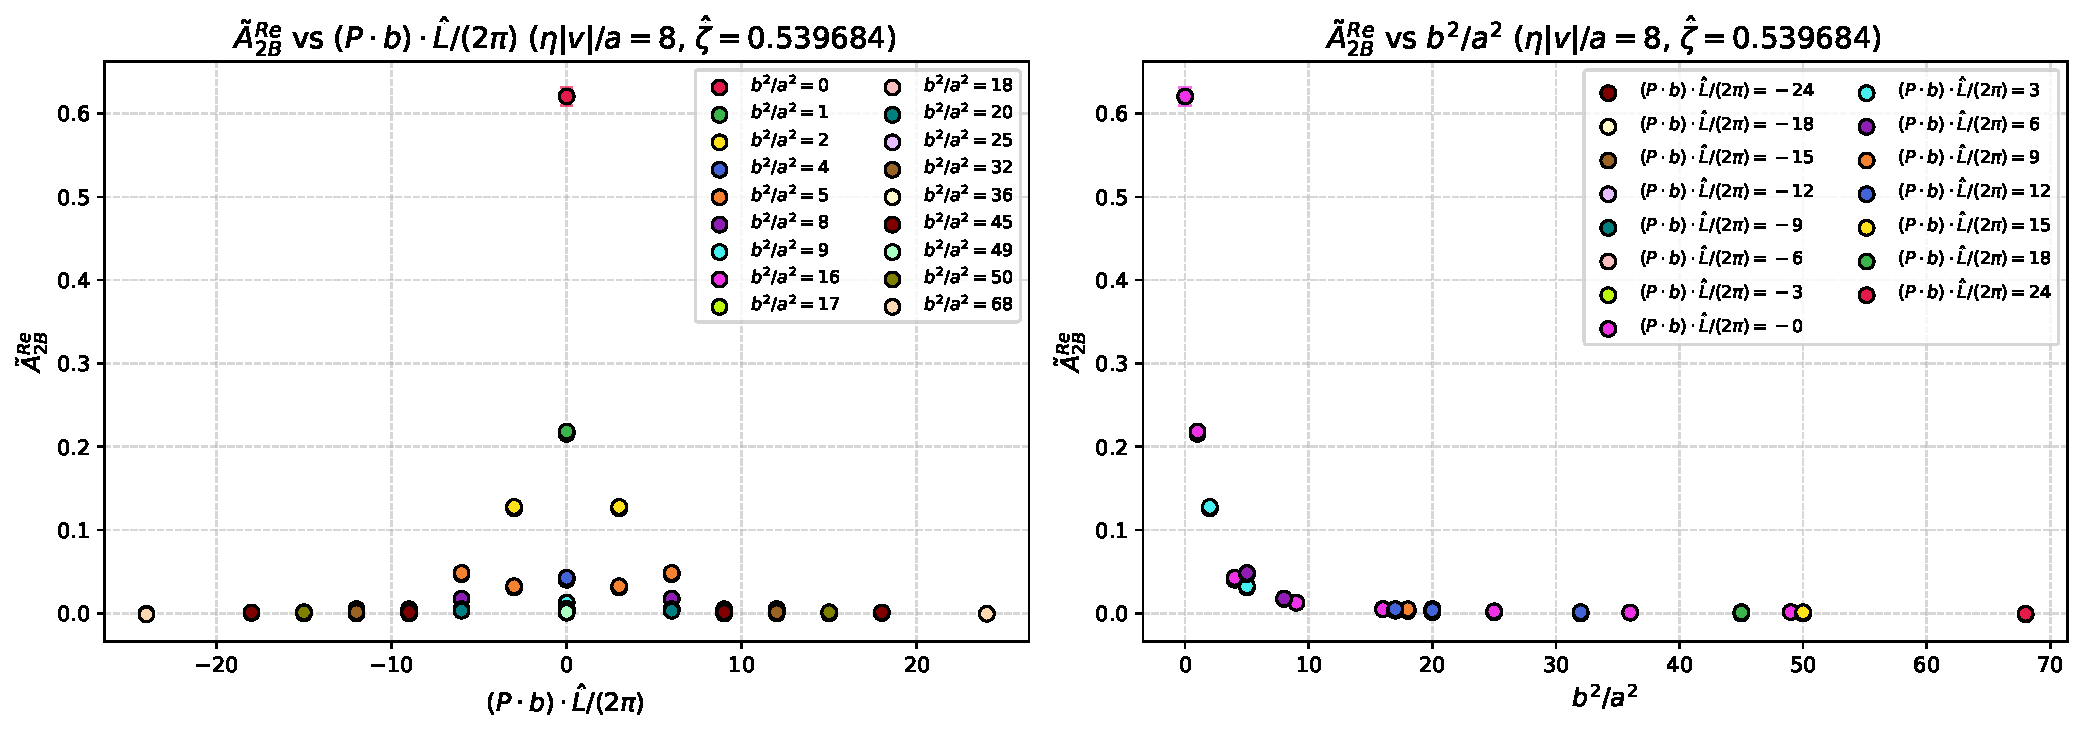
\includegraphics[height=0.38\textheight, trim=0 0 500 0, clip]{ReA2B_Pb_bsq_eta8_PL-3_2D.pdf} &
    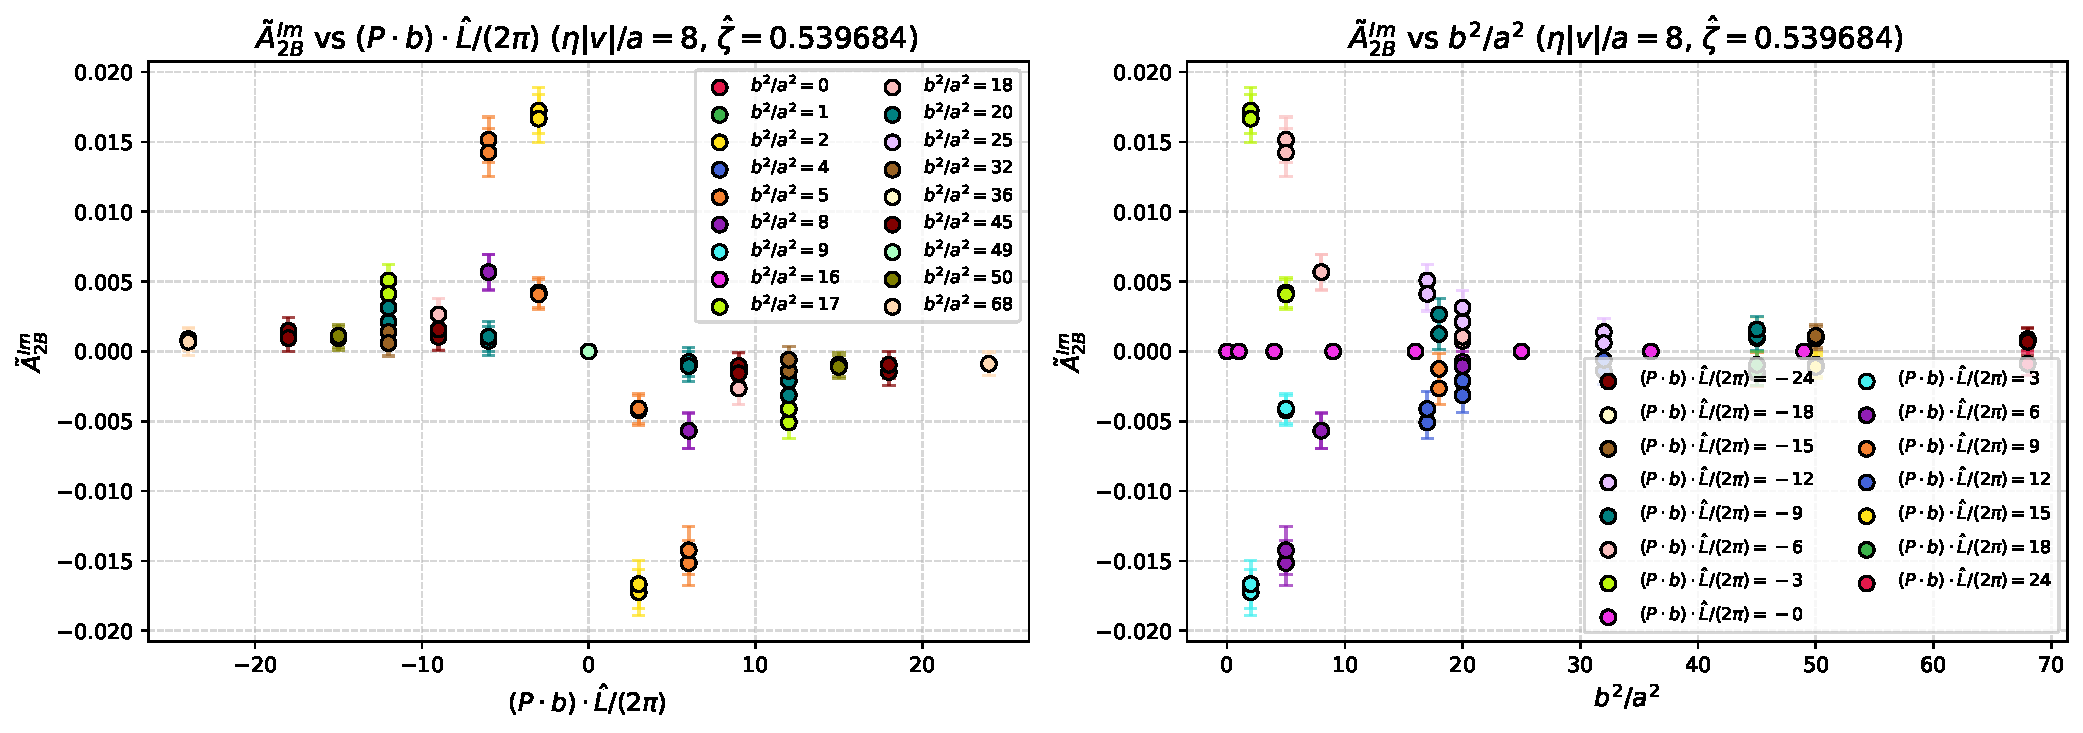
\includegraphics[height=0.38\textheight, trim=0 0 500 0, clip]{ImA2B_Pb_bsq_eta8_PL-3_2D.pdf} \\
    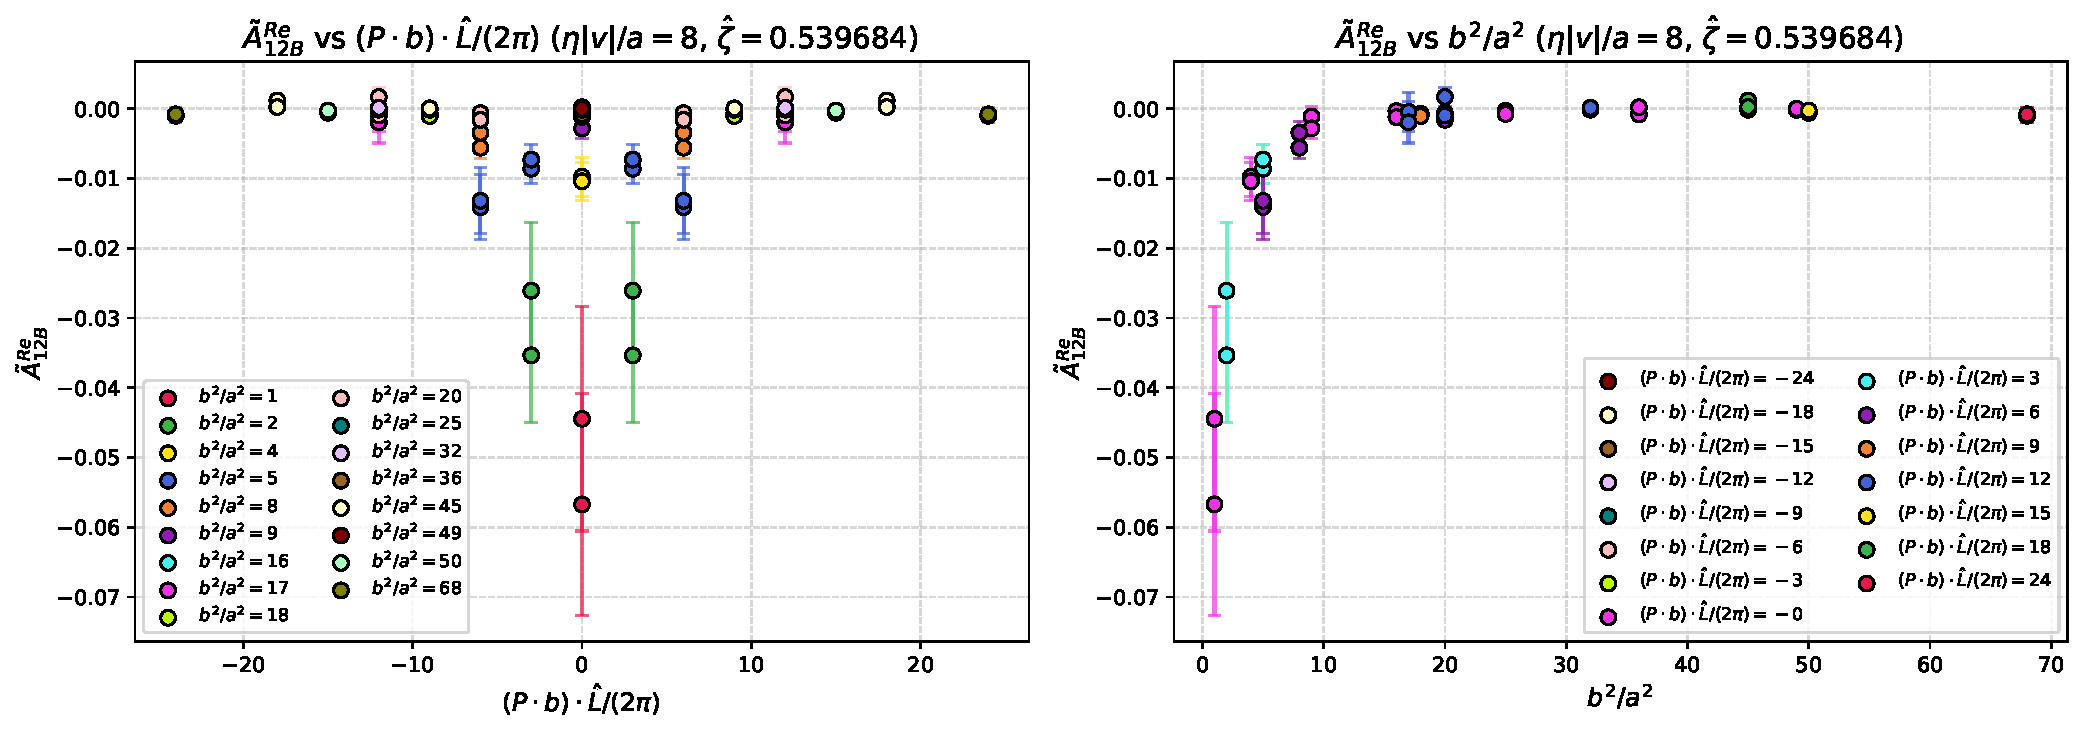
\includegraphics[height=0.38\textheight, trim=0 0 500 0, clip]{ReA12B_Pb_bsq_eta8_PL-3_2D.pdf} &
    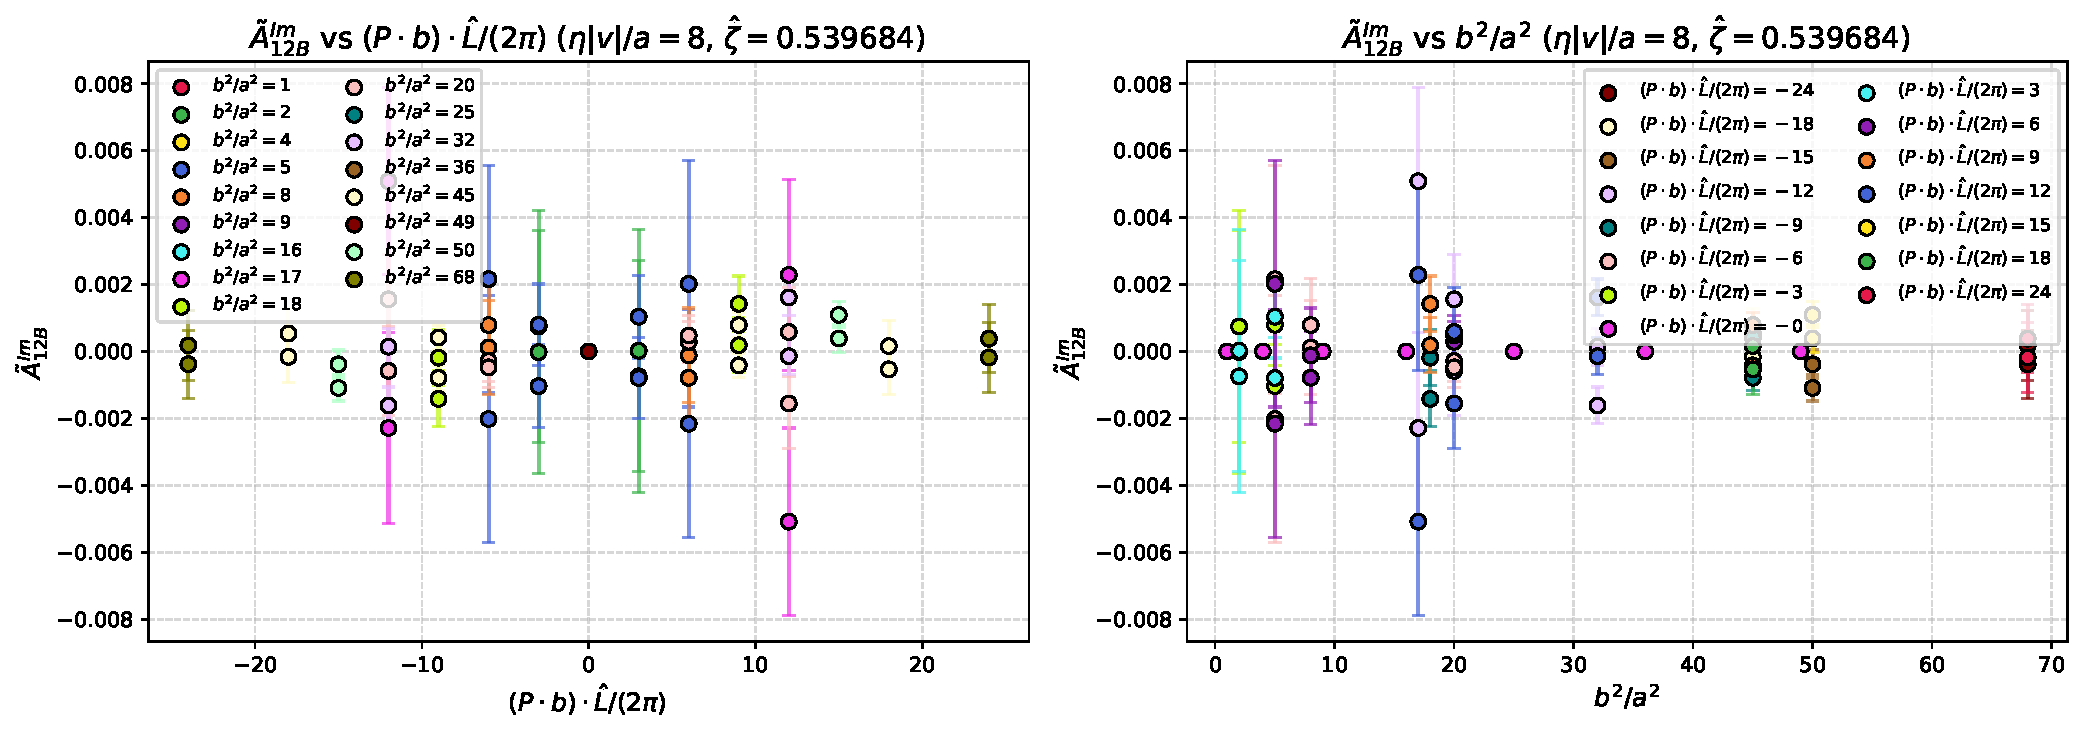
\includegraphics[height=0.38\textheight, trim=0 0 500 0, clip]{ImA12B_Pb_bsq_eta8_PL-3_2D.pdf}
  \end{tabular}
\end{frame}

% B1
\begin{frame}{Backup: lattice ensemble and $\zetahat$ at $P_L=-1$}
  \begin{columns}[t]
    \begin{column}{0.48\textwidth}
      \begin{block}{From the thesis}
        \begin{itemize}
          \item $n_f=2+1$ clover-improved Wilson fermions (Yoon \emph{et al.} 2017)
          \item $\hat L^3\times\hat T = 32^3\times 96$, \ $a=0.11403$ fm, \ $L\approx3.65$ fm
          \item $m_\pi=317$ MeV
          \item $\mN = 0.6228(28)/a = 1077.8(48)$ MeV
          \item $P_1=-2\pi/L=-339.8$ MeV
          \item Isovector $u-d$, connected contractions
        \end{itemize}
      \end{block}
      % TODO(Hari): m_pi, number of configurations and Jackknife bins, t_snk - t_src, smearing are not stated in the thesis
    \end{column}
    \begin{column}{0.50\textwidth}
      Setting the bracket of the constraint to zero:
      \[ \zetahat =\sqrt{\frac{P_{1}^2}{\mN^{2}\left(\frac{\mN^{2}}{P_{1}^{2}}+2\right)}} = \pm 0.090772 \]
      \[ \zetahat=\frac{-v_{1}P_{1}}{\sqrt{v_{1}^{2}+v_{3}^{2}}\ \mN} \ \Rightarrow\ v_{1}=\pm 0.301\,v_{3} \]
    \end{column}
  \end{columns}
\end{frame}

% B3
\begin{frame}{Backup: the $|\vect b|\ge3a$ cut for $\tAmp_{12B}^{\text{Re}}$}
  \vspace{2mm}
  \centering
  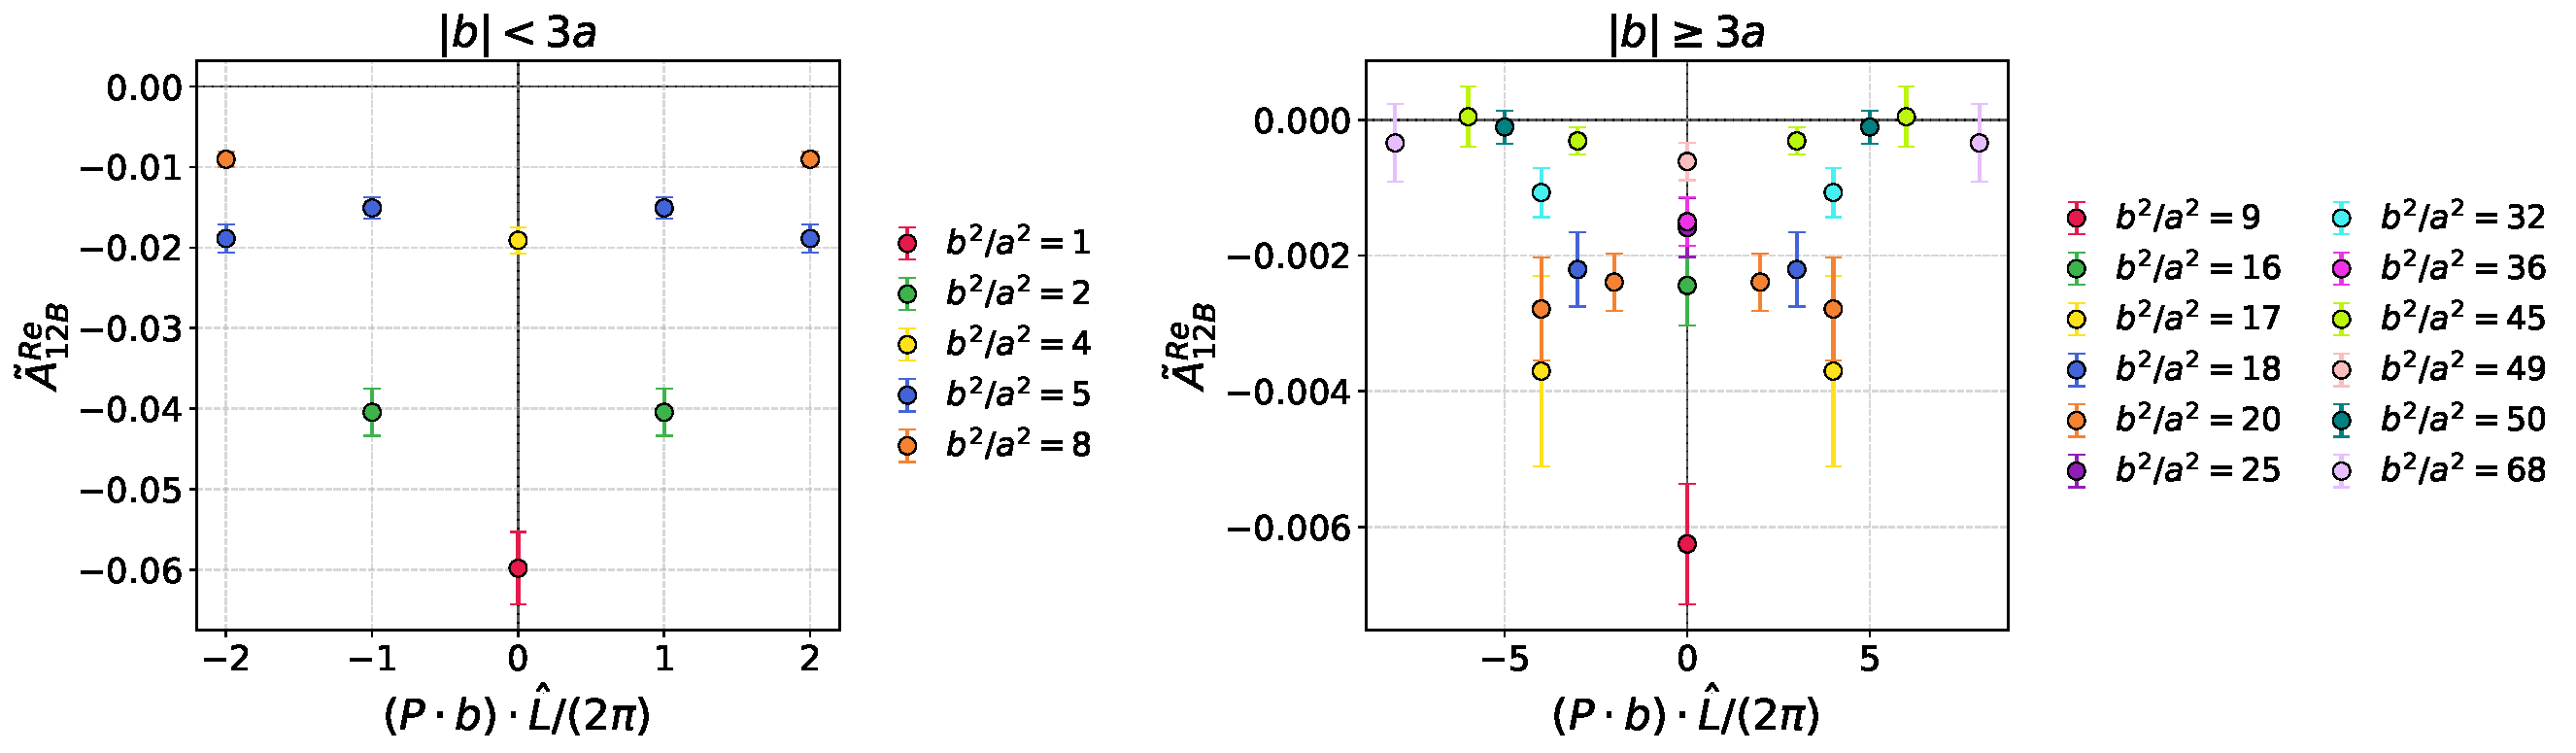
\includegraphics[width=\linewidth]{A12B_Re_b_lessthan3_and_ge3.pdf}
\end{frame}

% B3b
\begin{frame}{Backup: $\tAmp_{12B}^{\text{Im}}$ is consistent with zero}
  \centering
  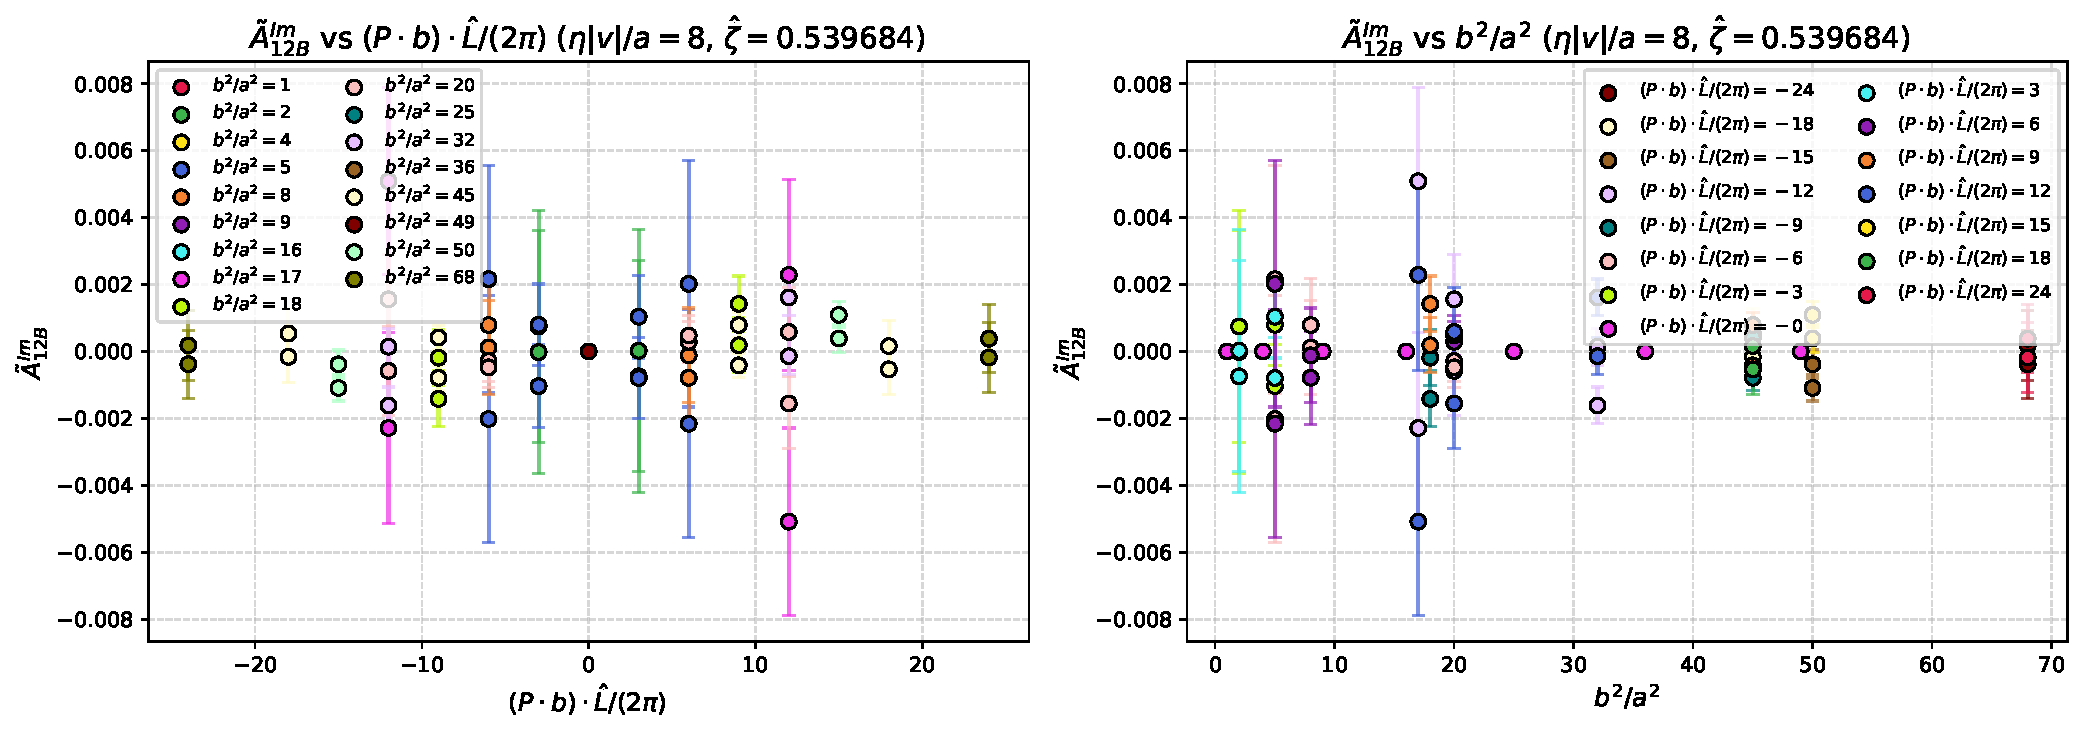
\includegraphics[width=\linewidth]{ImA12B_Pb_bsq_eta8_PL-3_2D.pdf}\\
  {\scriptsize $\tAmp_{12B}^{\text{Im}}$ at $P_L=-3$, $\eta|v|/a=8$ (all $b^2$, including $|\vect b|<3a$): consistent with zero, so dropped.}
\end{frame}

% B4
\begin{frame}{Backup: PySR benchmark fits}
  \begin{columns}[c]
    \begin{column}{0.62\textwidth}
      \centering
      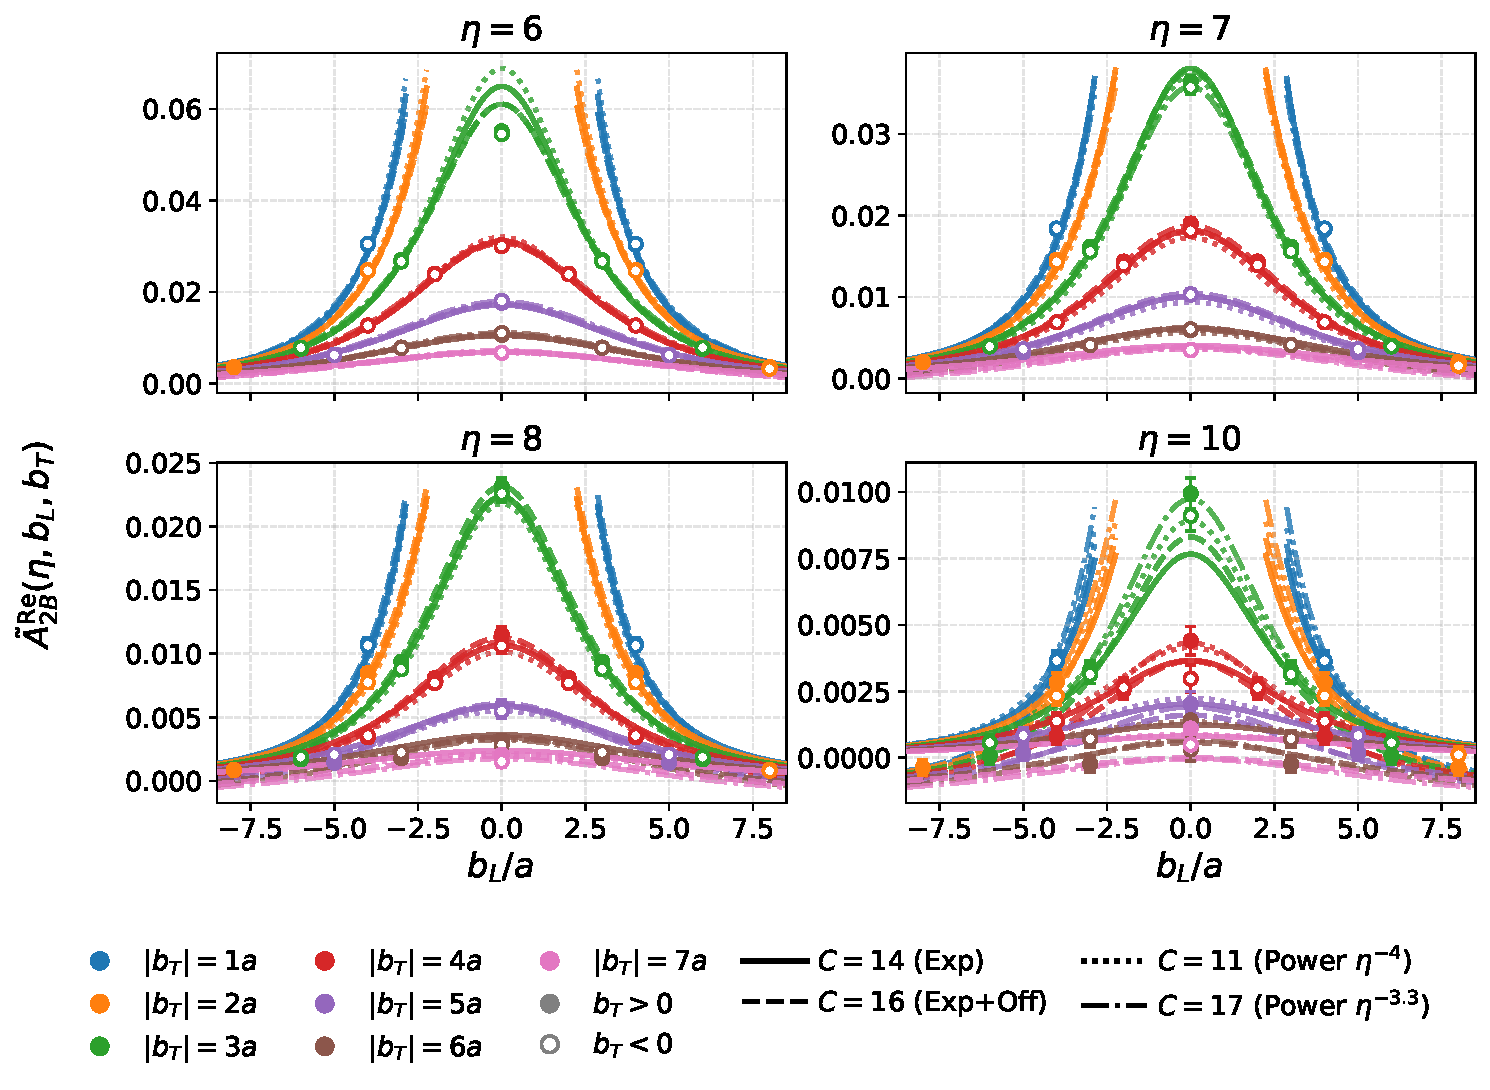
\includegraphics[height=0.8\textheight, width=\linewidth, keepaspectratio]{01_A2B_PySR_Benchmark_Fits.pdf}
    \end{column}
    \begin{column}{0.36\textwidth}
      \begin{itemize}
        \item Run on $\tAmp_{2B}^{\text{Re}}$ at $P_L=-1$ only.
        \item $\mathcal{P}_{\text{asymptotic}}$ sums $|\tAmp^{\text{model}}|$ at large $b_L$.
        \item Every formula with spatial dependence depends on $b_L, b_T$ only through $b^2$: a guide, not the final model.
      \end{itemize}
    \end{column}
  \end{columns}
\end{frame}

% B5
\begin{frame}{Backup: $c(\eta)$ candidates and the Fourier-transform width}
  \centering
  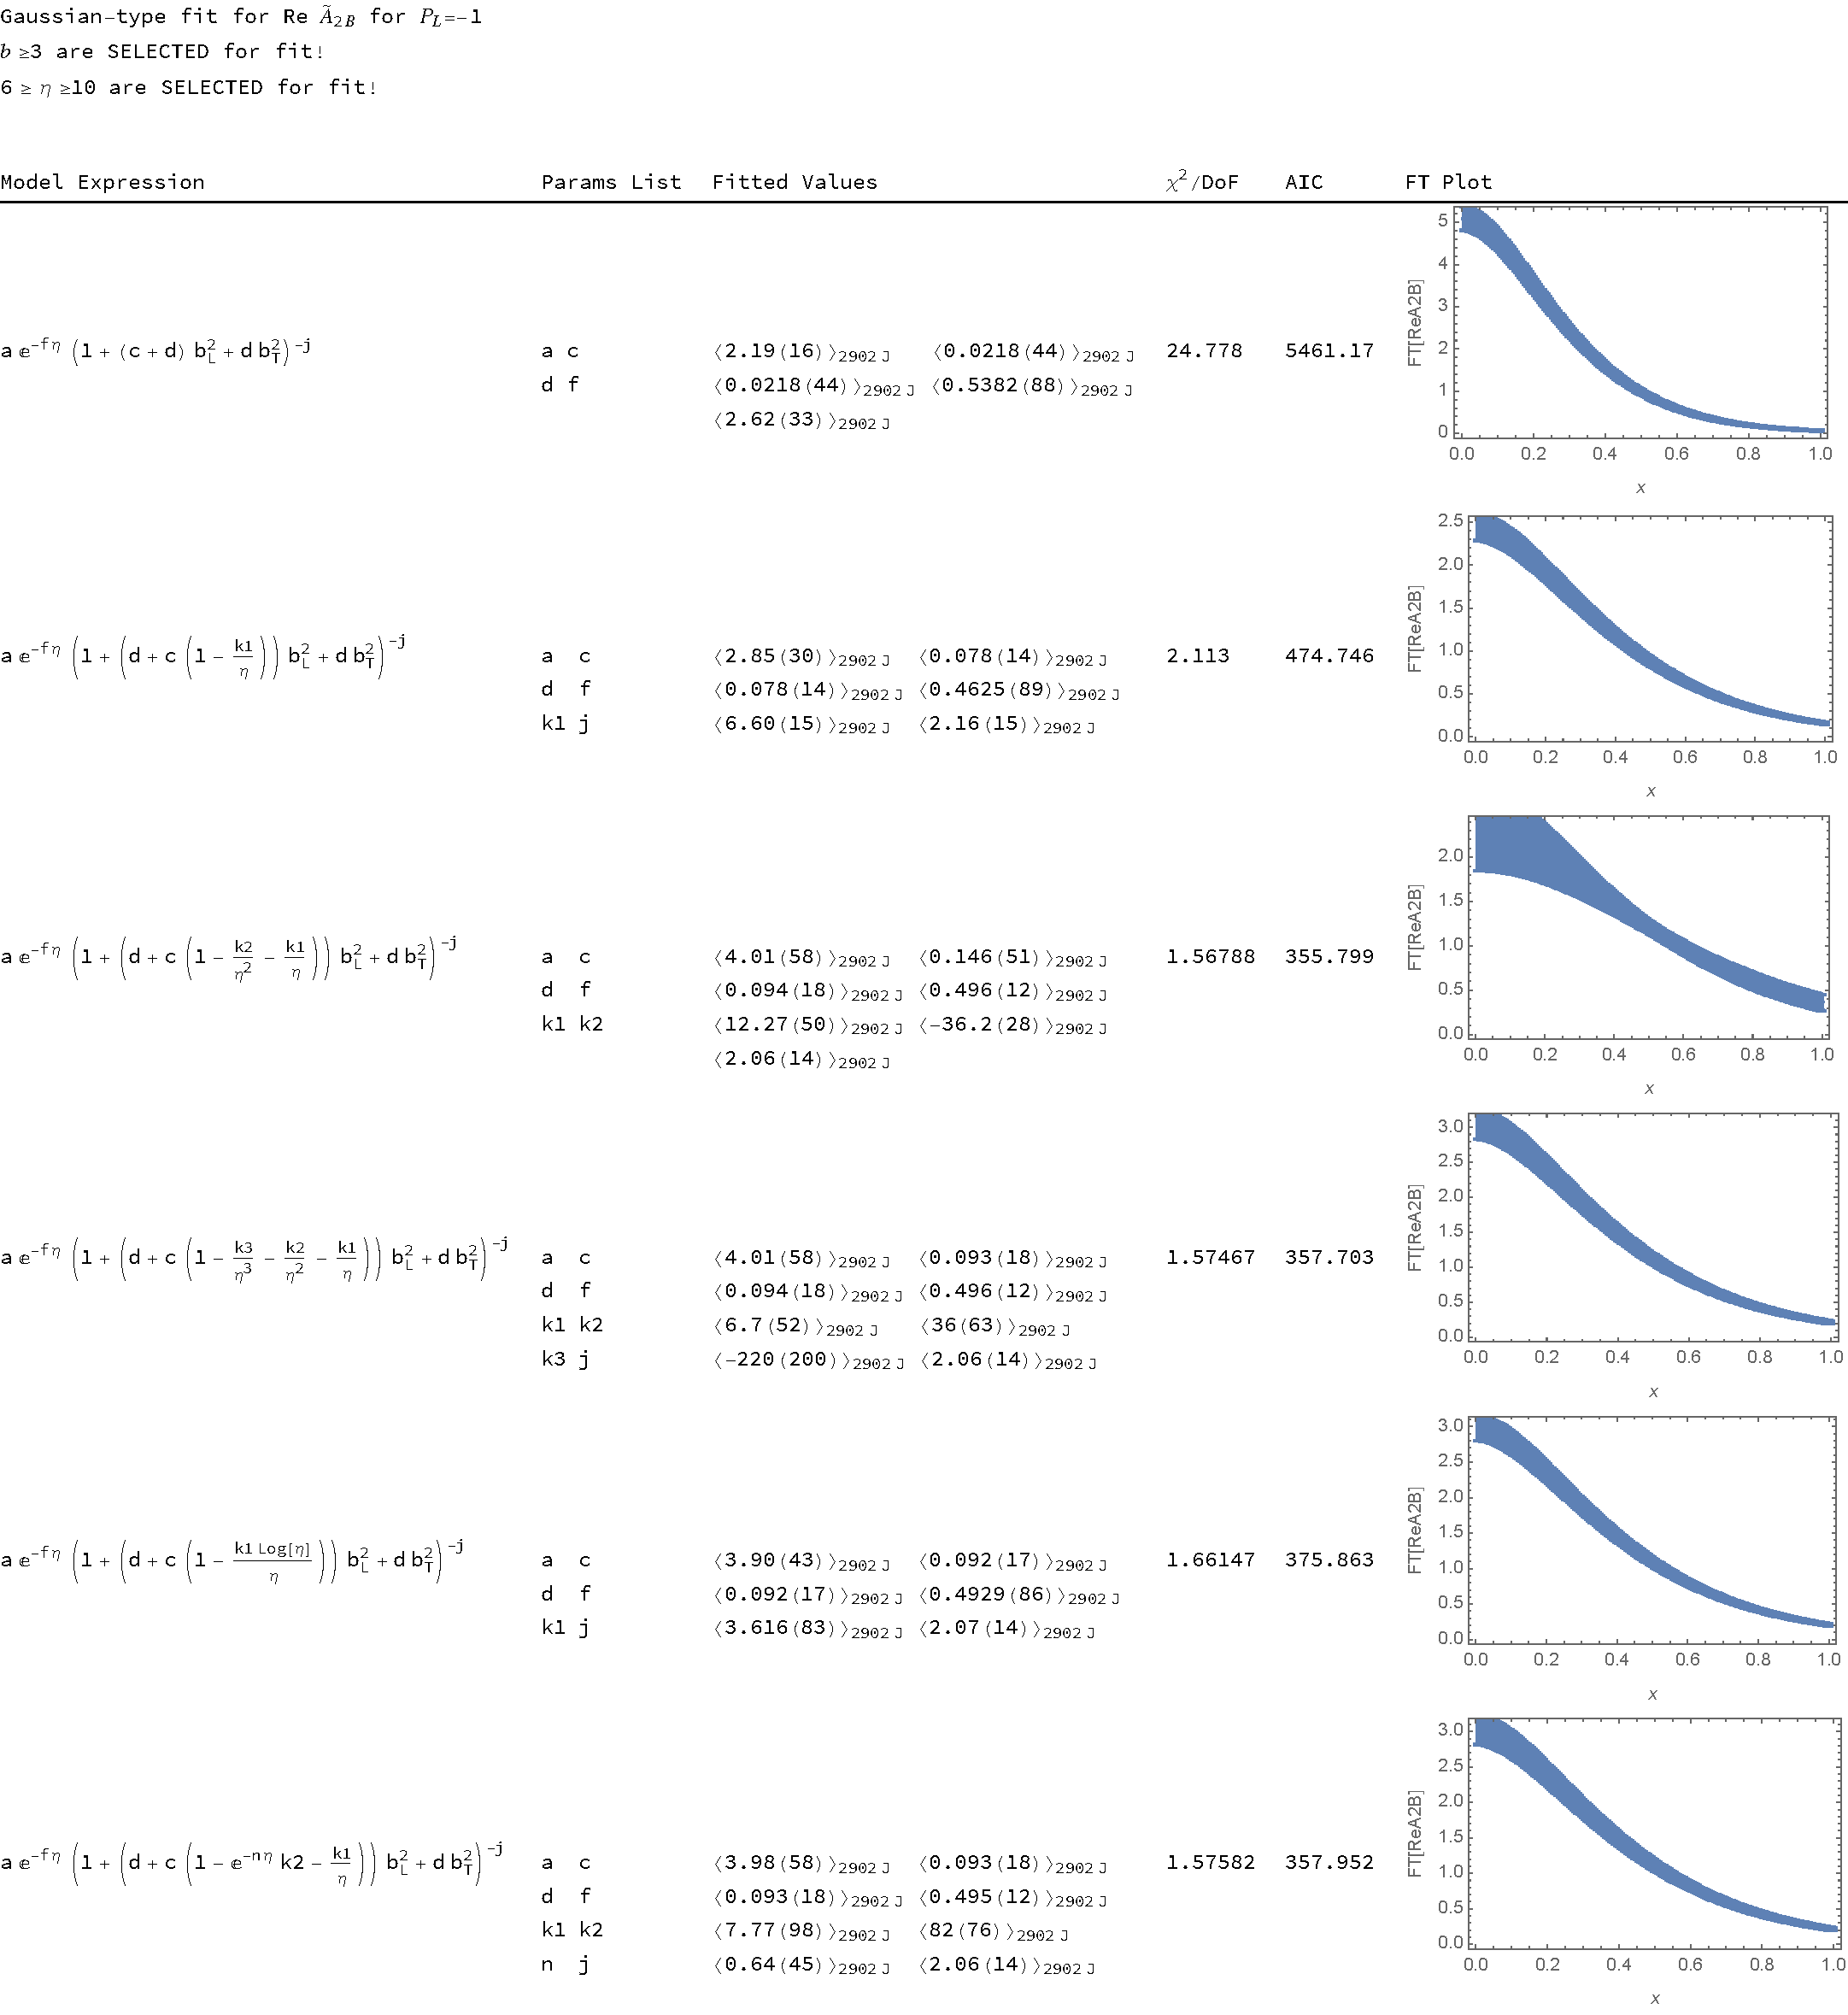
\includegraphics[height=0.82\textheight, keepaspectratio]{A2BfitFT_eta_Asymptotic_P1.pdf}
\end{frame}

% B5b
\begin{frame}{Backup: $\eta$-independence of $d$, and the $c(\eta)$ choice}
  \begin{columns}[c]
    \begin{column}{0.48\textwidth}
      \centering
      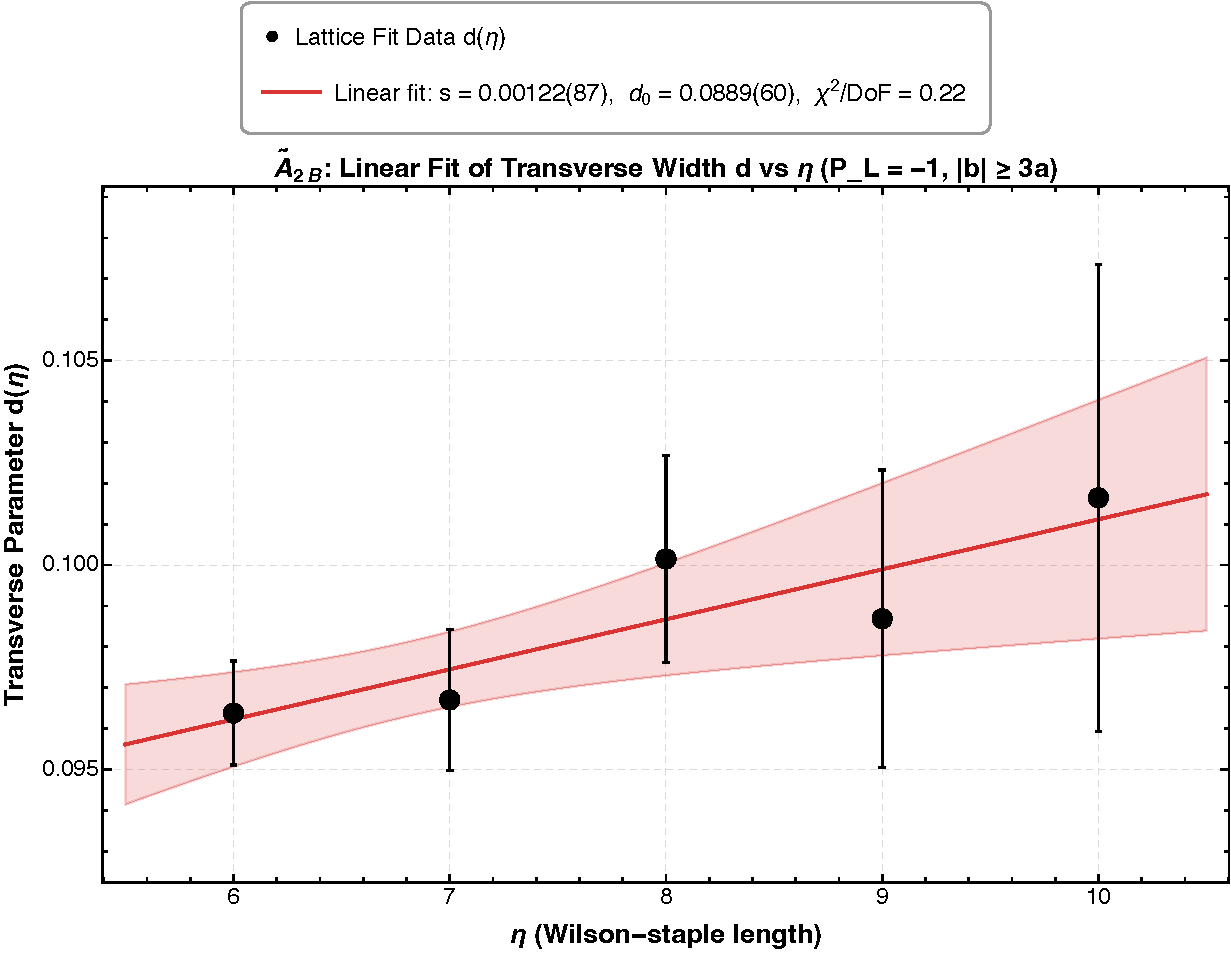
\includegraphics[width=0.9\linewidth]{A2B_d_eta_Independence_P1.pdf}\\
      {\scriptsize $d(\eta)$ for $\tAmp_{2B}^{\text{Re}}$: slope $0.00122(87)$}
    \end{column}
    \begin{column}{0.50\textwidth}
      \begin{itemize}
        \item The $x$-width of $\tAmp_{2B}^{\text{Re}}$ moves with the choice of $c(\eta)$ (previous slide).
        \item $c_2(\eta)=c\big(1-\tfrac{k_1}{\eta}-\tfrac{k_2}{\eta^2}\big)$: lowest AIC, suppresses antiquarks at $x\lesssim-0.2$, consistent with the $x$-integrated results.
        \item The $b_L^2$ coefficient is $d+c_2(\eta)$, which stays positive over $\eta\in[6,10]$.
        % TODO(Hari): state how c(eta) with k1,k2 enters the transform and the zeta-hat extrapolation
      \end{itemize}
    \end{column}
  \end{columns}
\end{frame}

% B6
\begin{frame}{Backup: integrability of the power-law models (remarks, not in thesis)}
  \begin{itemize}
    \item Even amplitudes: $\big[1+C\,(P\cdot b)^2+\ldots\big]^{-j}\sim|P\cdot b|^{-2j}$ $\Rightarrow$ absolutely integrable for $j>1/2$.
    \item $\tAmp_{2B}^{\text{Im}}\propto b_L\,[\ldots]^{-j}\sim|P\cdot b|^{1-2j}$ $\Rightarrow$ absolutely integrable only for $j>1$.
    \item $j_{\text{im}}$ at the simulated momenta $P_L=-1,-2,-3,-4$: \ $1.108(21)$, $1.141(20)$, $1.057(15)$, $1.0084(79)$, all $>1$.
    \item Extrapolated to $\zetahat\to\infty$:
  \end{itemize}
  \[ j_{\text{re}} = 2.0667(69), \quad j_{\text{im}} = 0.9921(92), \quad j_{\text{reA12B}} = 2.0026(40) \]
  \begin{itemize}
    \item At $j_{\text{im}}\approx1$ the sine transform converges only conditionally; this is the sharp structure of $\tAmp_{2B}^{[x]\text{Im}}$ near $x=0$.
    \item Power laws are not entire functions, so support extends beyond $|x|\le1$; numerically $\int_{-\infty}^{\infty}$ and $\int_{-1}^{1}$ agree within errors (next slide).
  \end{itemize}
\end{frame}

% B7
\begin{frame}{Backup: $x$-integrals at $\zetahat\to\infty$, $|\vprp b|=3a$}
  \centering
  \renewcommand{\arraystretch}{1.5}
  {\small
  \begin{tabular}{lcccc}
    \toprule
    Integral & $[-\infty, \infty]$ & $[-1, 1]$ & $[-1, 0]$ & $[0, 1]$ \\
    \midrule
    $\int dx\, \tAmp^{[x]\text{Re}}_{2B}$ & $0.751(79)$ & $0.751(80)$ & $0.375(40)$ & $0.375(40)$ \\
    $\int dx\, \tAmp^{[x]\text{Im}}_{2B}$ & $6(96)\times10^{-17}$ & $3(24)\times10^{-16}$ & $0.165(27)$ & $-0.169(29)$ \\
    $\int dx\, \tilde{f}_1^{(0)}$ & $1.50(16)$ & $1.50(16)$ & $0.421(81)$ & $1.09(11)$  \\
    $\int dx\, \tilde{f}_{1T}^{\perp(1)}$ & $0.302(53)$ & $0.302(53)$ & $0.151(27)$ & $0.151(27)$ \\
    $\mN \int dx\, \tilde{f}_{1T}^{\perp(1)} / \int dx\, \tilde{f}_1^{(0)}$ & $0.217(38)$ & $0.217(38)$ & $0.387(89)$ & $0.150(26)$ \\
    \bottomrule
  \end{tabular}}
  \raggedright
  \begin{itemize}
    \item First four rows are unrenormalized; only the ratio (last row) is quoted as a physical quantity.
    \item The $(-\infty,\infty)$ ratio (last row) equals the $\bvec\tcdot P=0$ ratio (an identity). The content is the split into $[-1,0]$ and $[0,1]$.
  \end{itemize}
\end{frame}

% B8
\begin{frame}{Backup: all twelve parameter extrapolations}
  \centering
  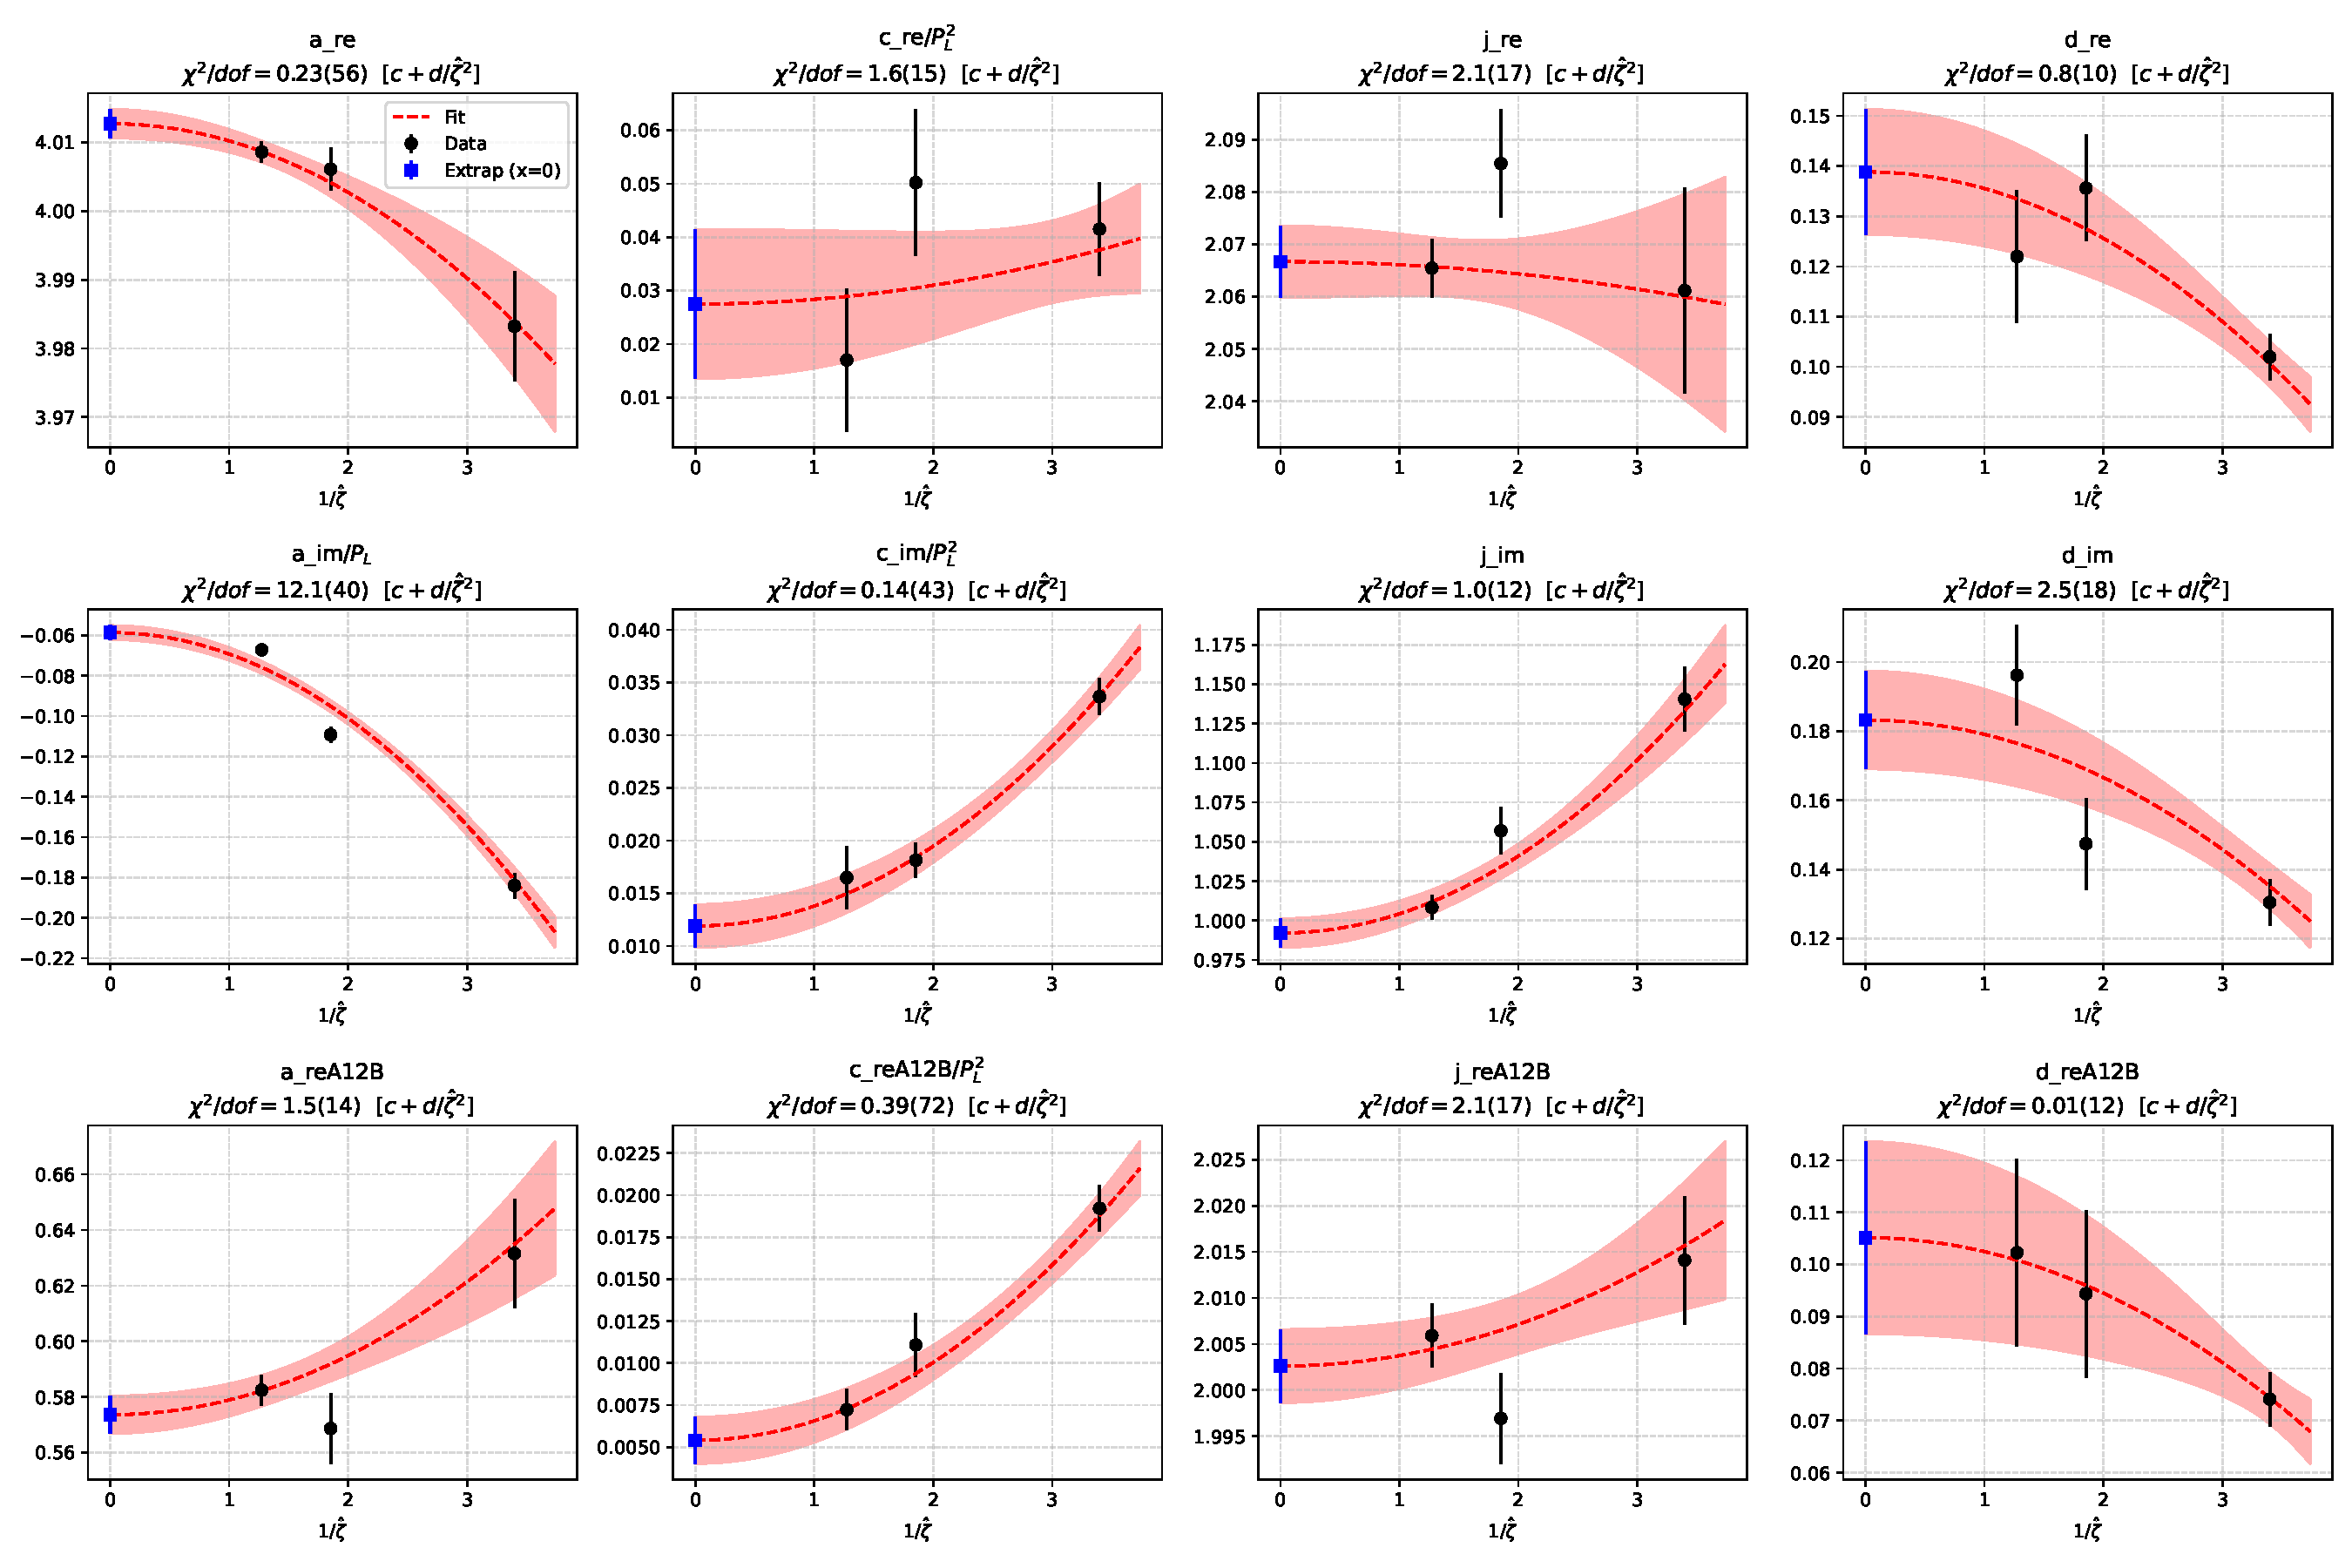
\includegraphics[height=0.8\textheight, keepaspectratio]{Param_Extrapolations_1byZetahat_sq_P234_bmin3_eta610_b29.0.pdf}\\
  {\scriptsize Rows: $\tAmp_{2B}^{\text{Re}}$, $\tAmp_{2B}^{\text{Im}}$, $\tAmp_{12B}^{\text{Re}}$. Each fit: 3 points, 2 parameters.}
\end{frame}

% B9
\begin{frame}{Backup: Sivers shift at the four momenta vs $1/\zetahat$}
  \centering
  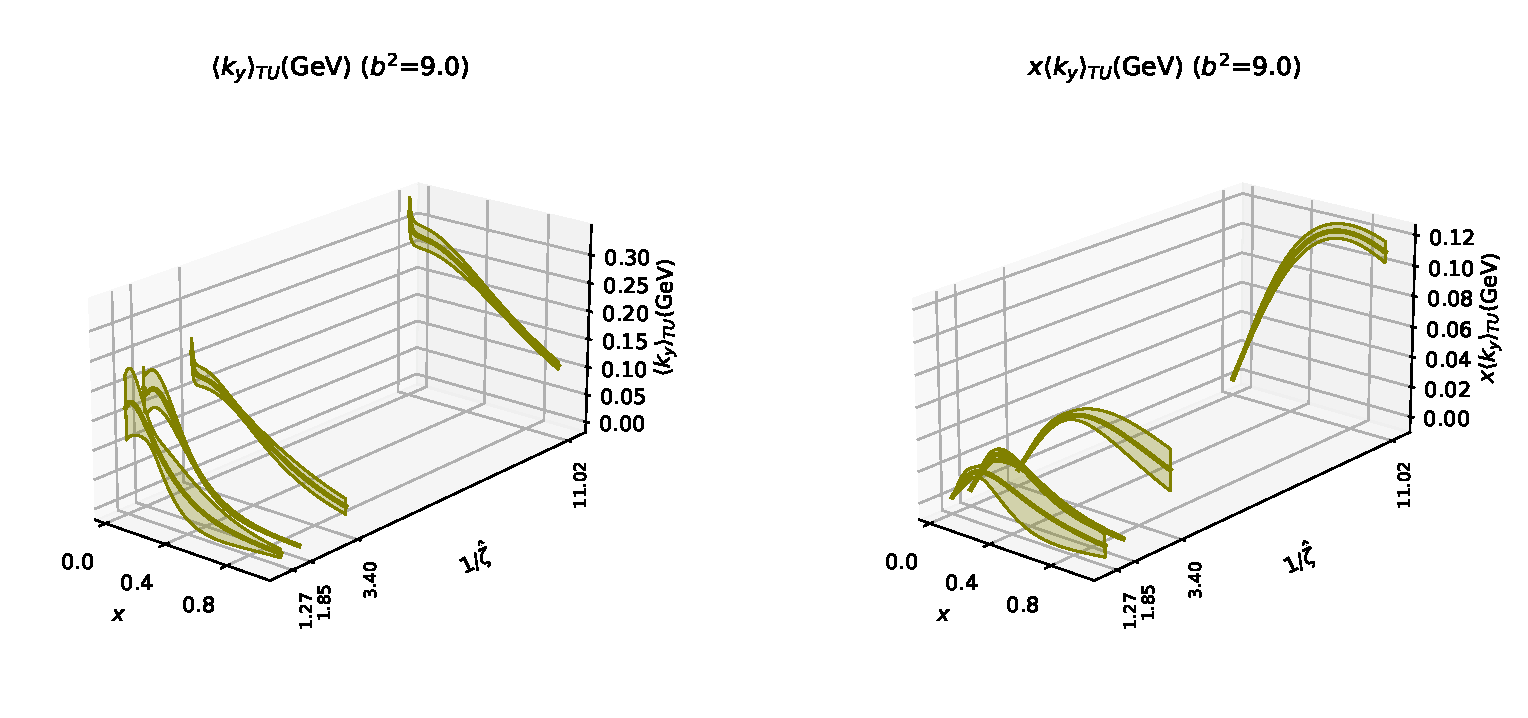
\includegraphics[width=0.9\linewidth]{SimulFit_Distinct_1_over_PL_bmin3_eta610_b29.0_Sivers.pdf}
\end{frame}

% B10
\begin{frame}{Backup: extrapolated amplitudes and TMDs}
  \centering
  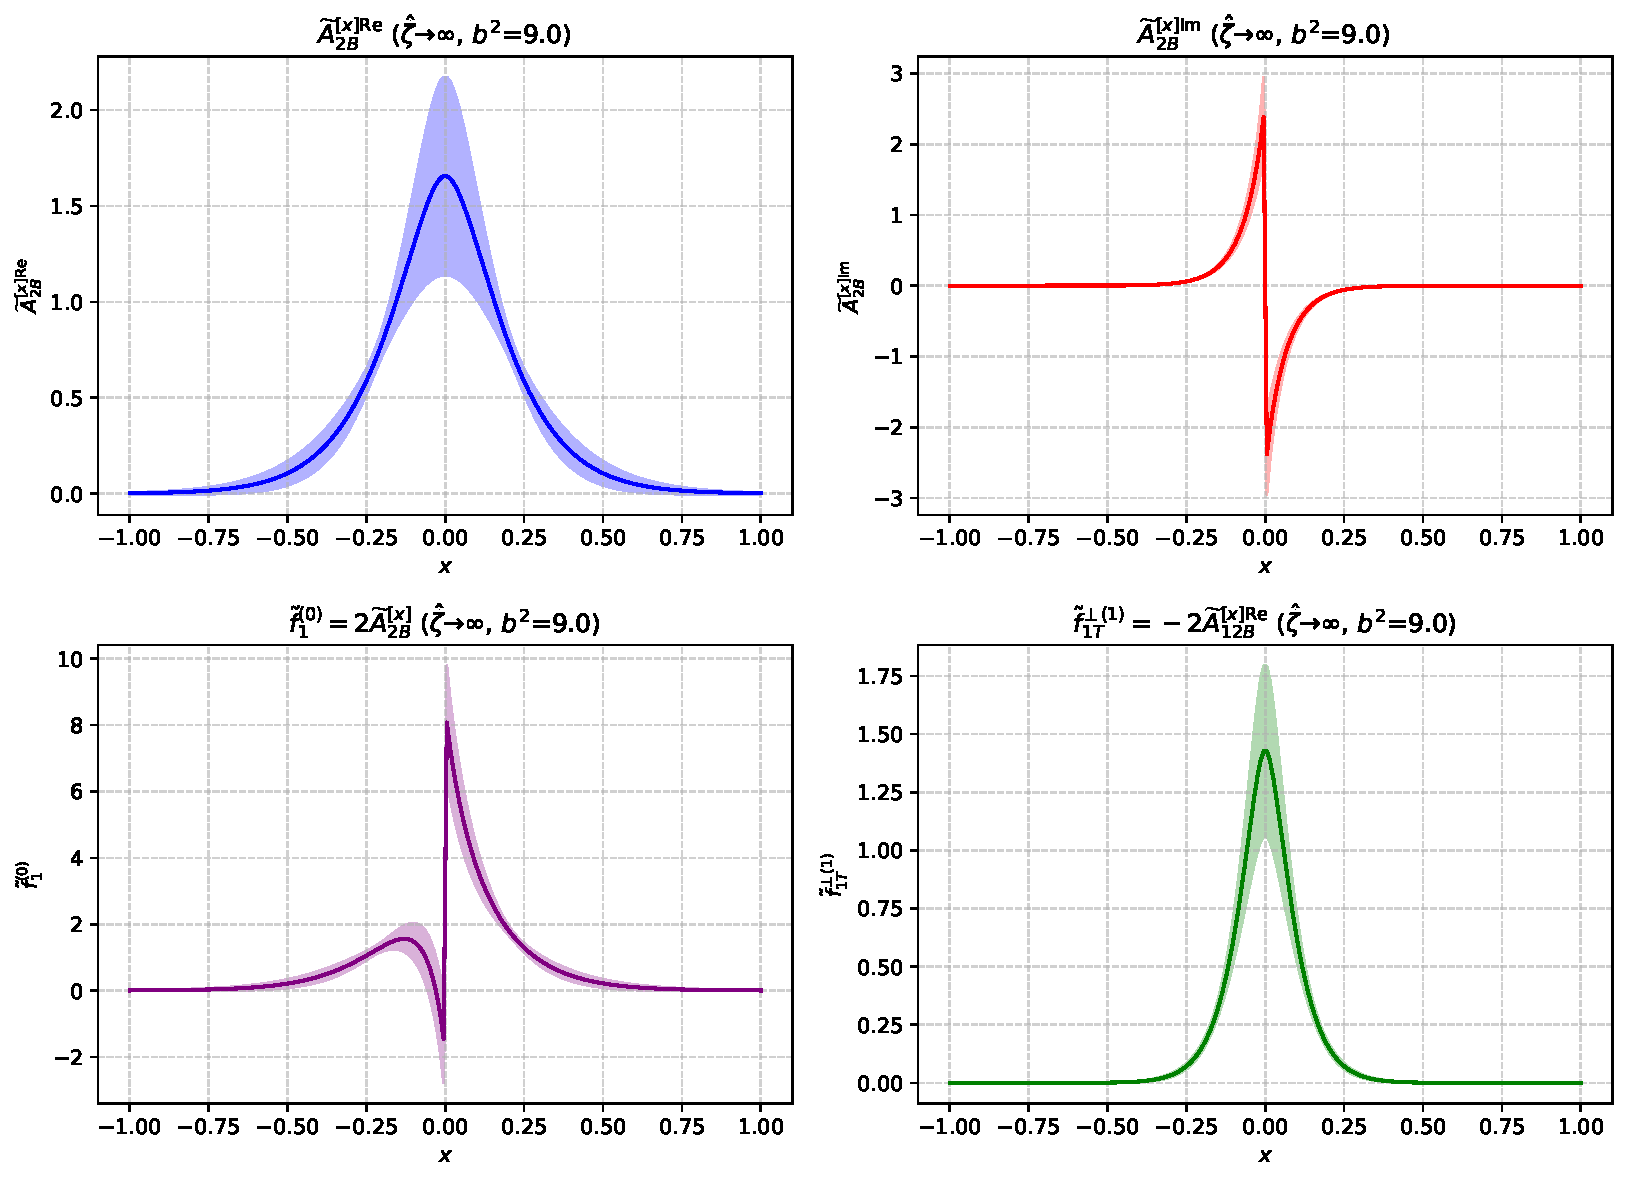
\includegraphics[height=0.82\textheight, keepaspectratio]{Extrapolated_AmpLevel_P234_Sivers_1_over_zetahat_sq_bmin3_eta610_b29.0_Amps.pdf}
\end{frame}

% B11
\begin{frame}{Backup: full $x$-dependence at $P_L=-3$}
  \centering
  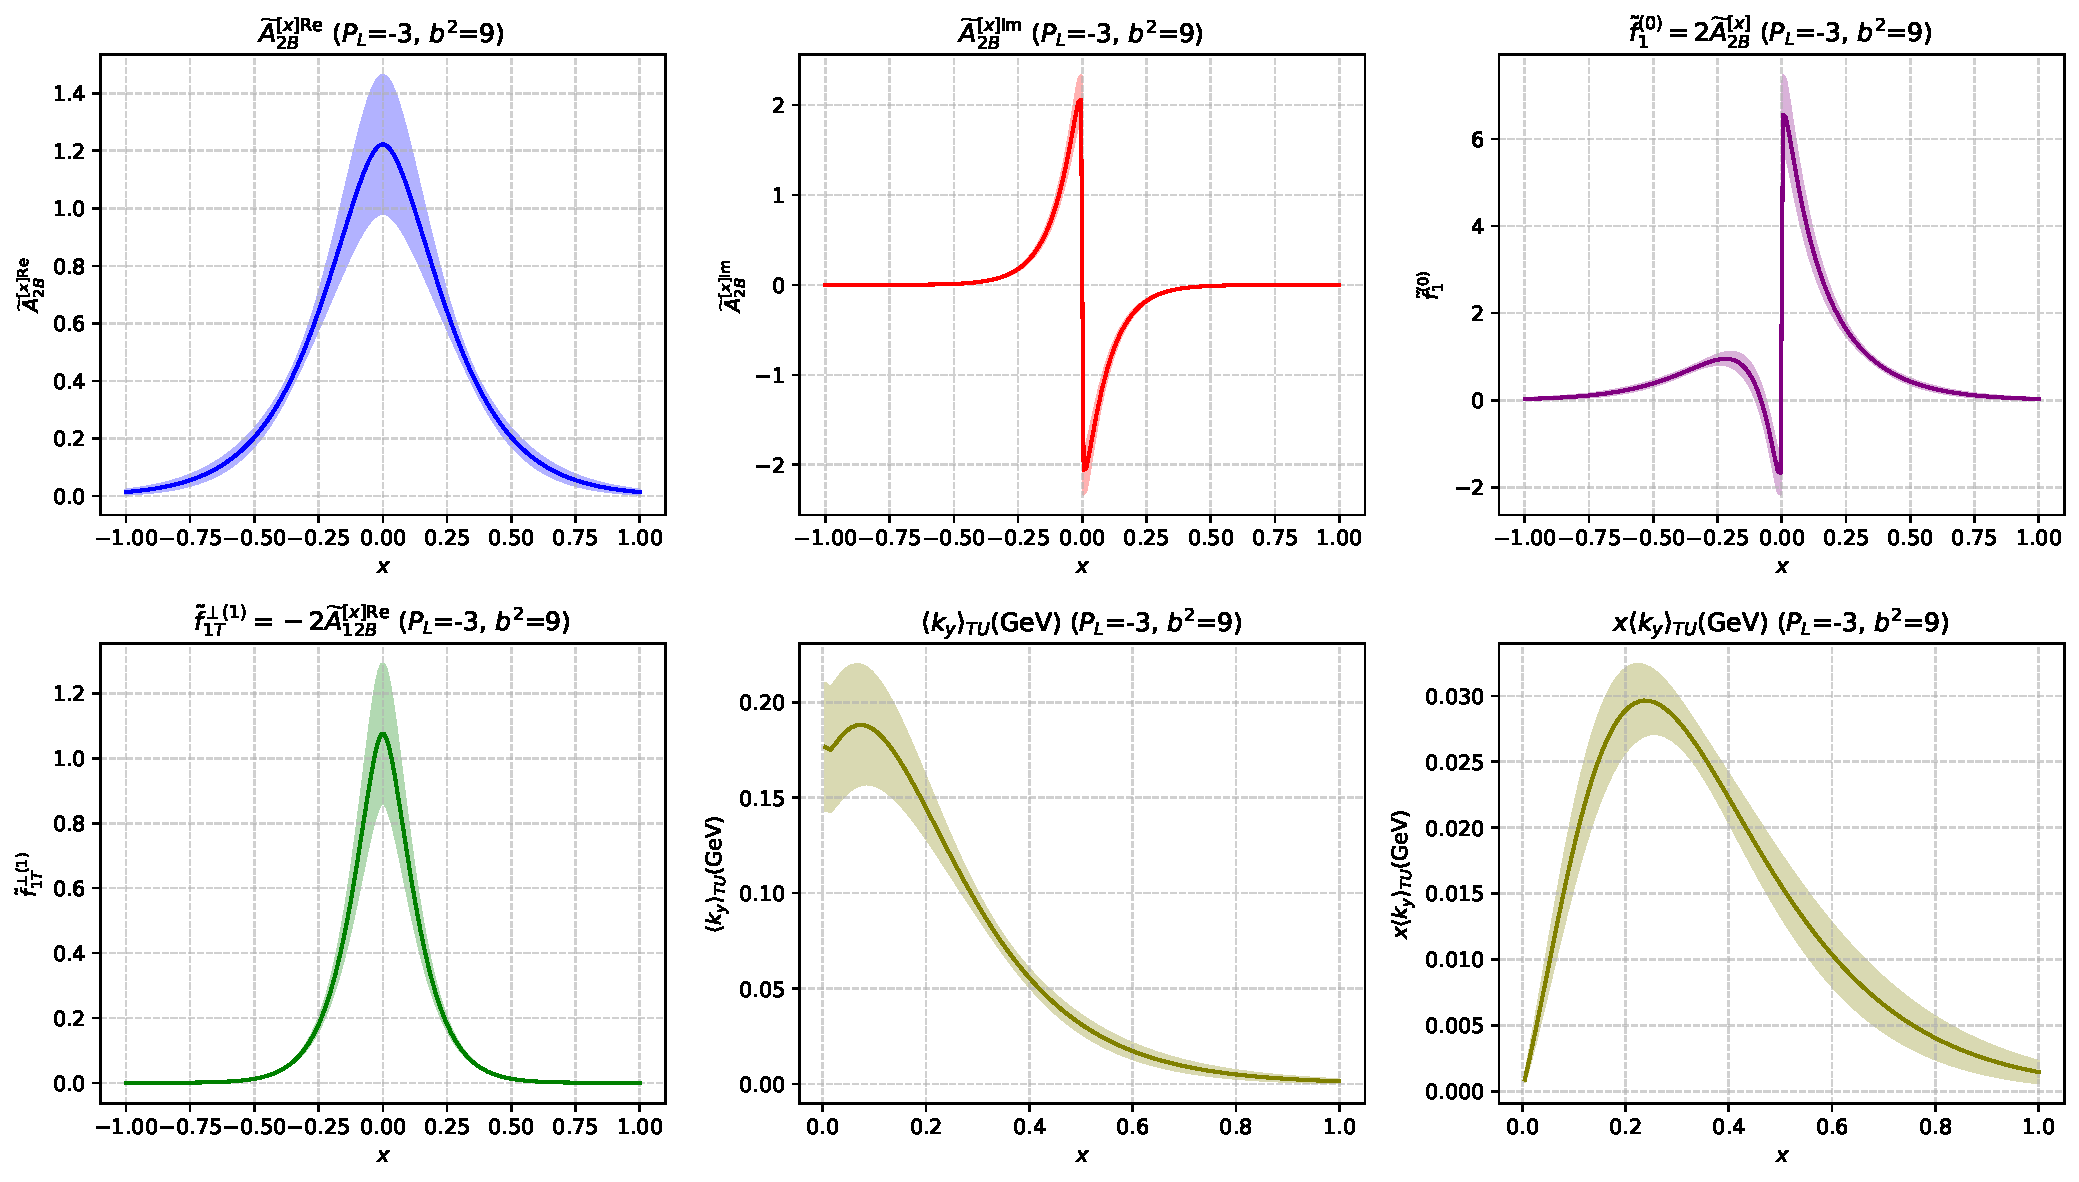
\includegraphics[width=0.75\linewidth]{FT_xdep_A2B_A12B_bmin3_eta610_b2-9_PL-3.pdf}\\
  {\scriptsize Top: $\tAmp^{[x]\text{Re}}_{2B}$, $\tAmp^{[x]\text{Im}}_{2B}$, $\tilde f_1^{(0)}$. Bottom: $\tilde f_{1T}^{\perp(1)}$, $\langle k_y\rangle_{TU}$, $x\langle k_y\rangle_{TU}$.}
\end{frame}

% B12
\begin{frame}{Backup: global fit at $P_L=-3$}
  \centering
  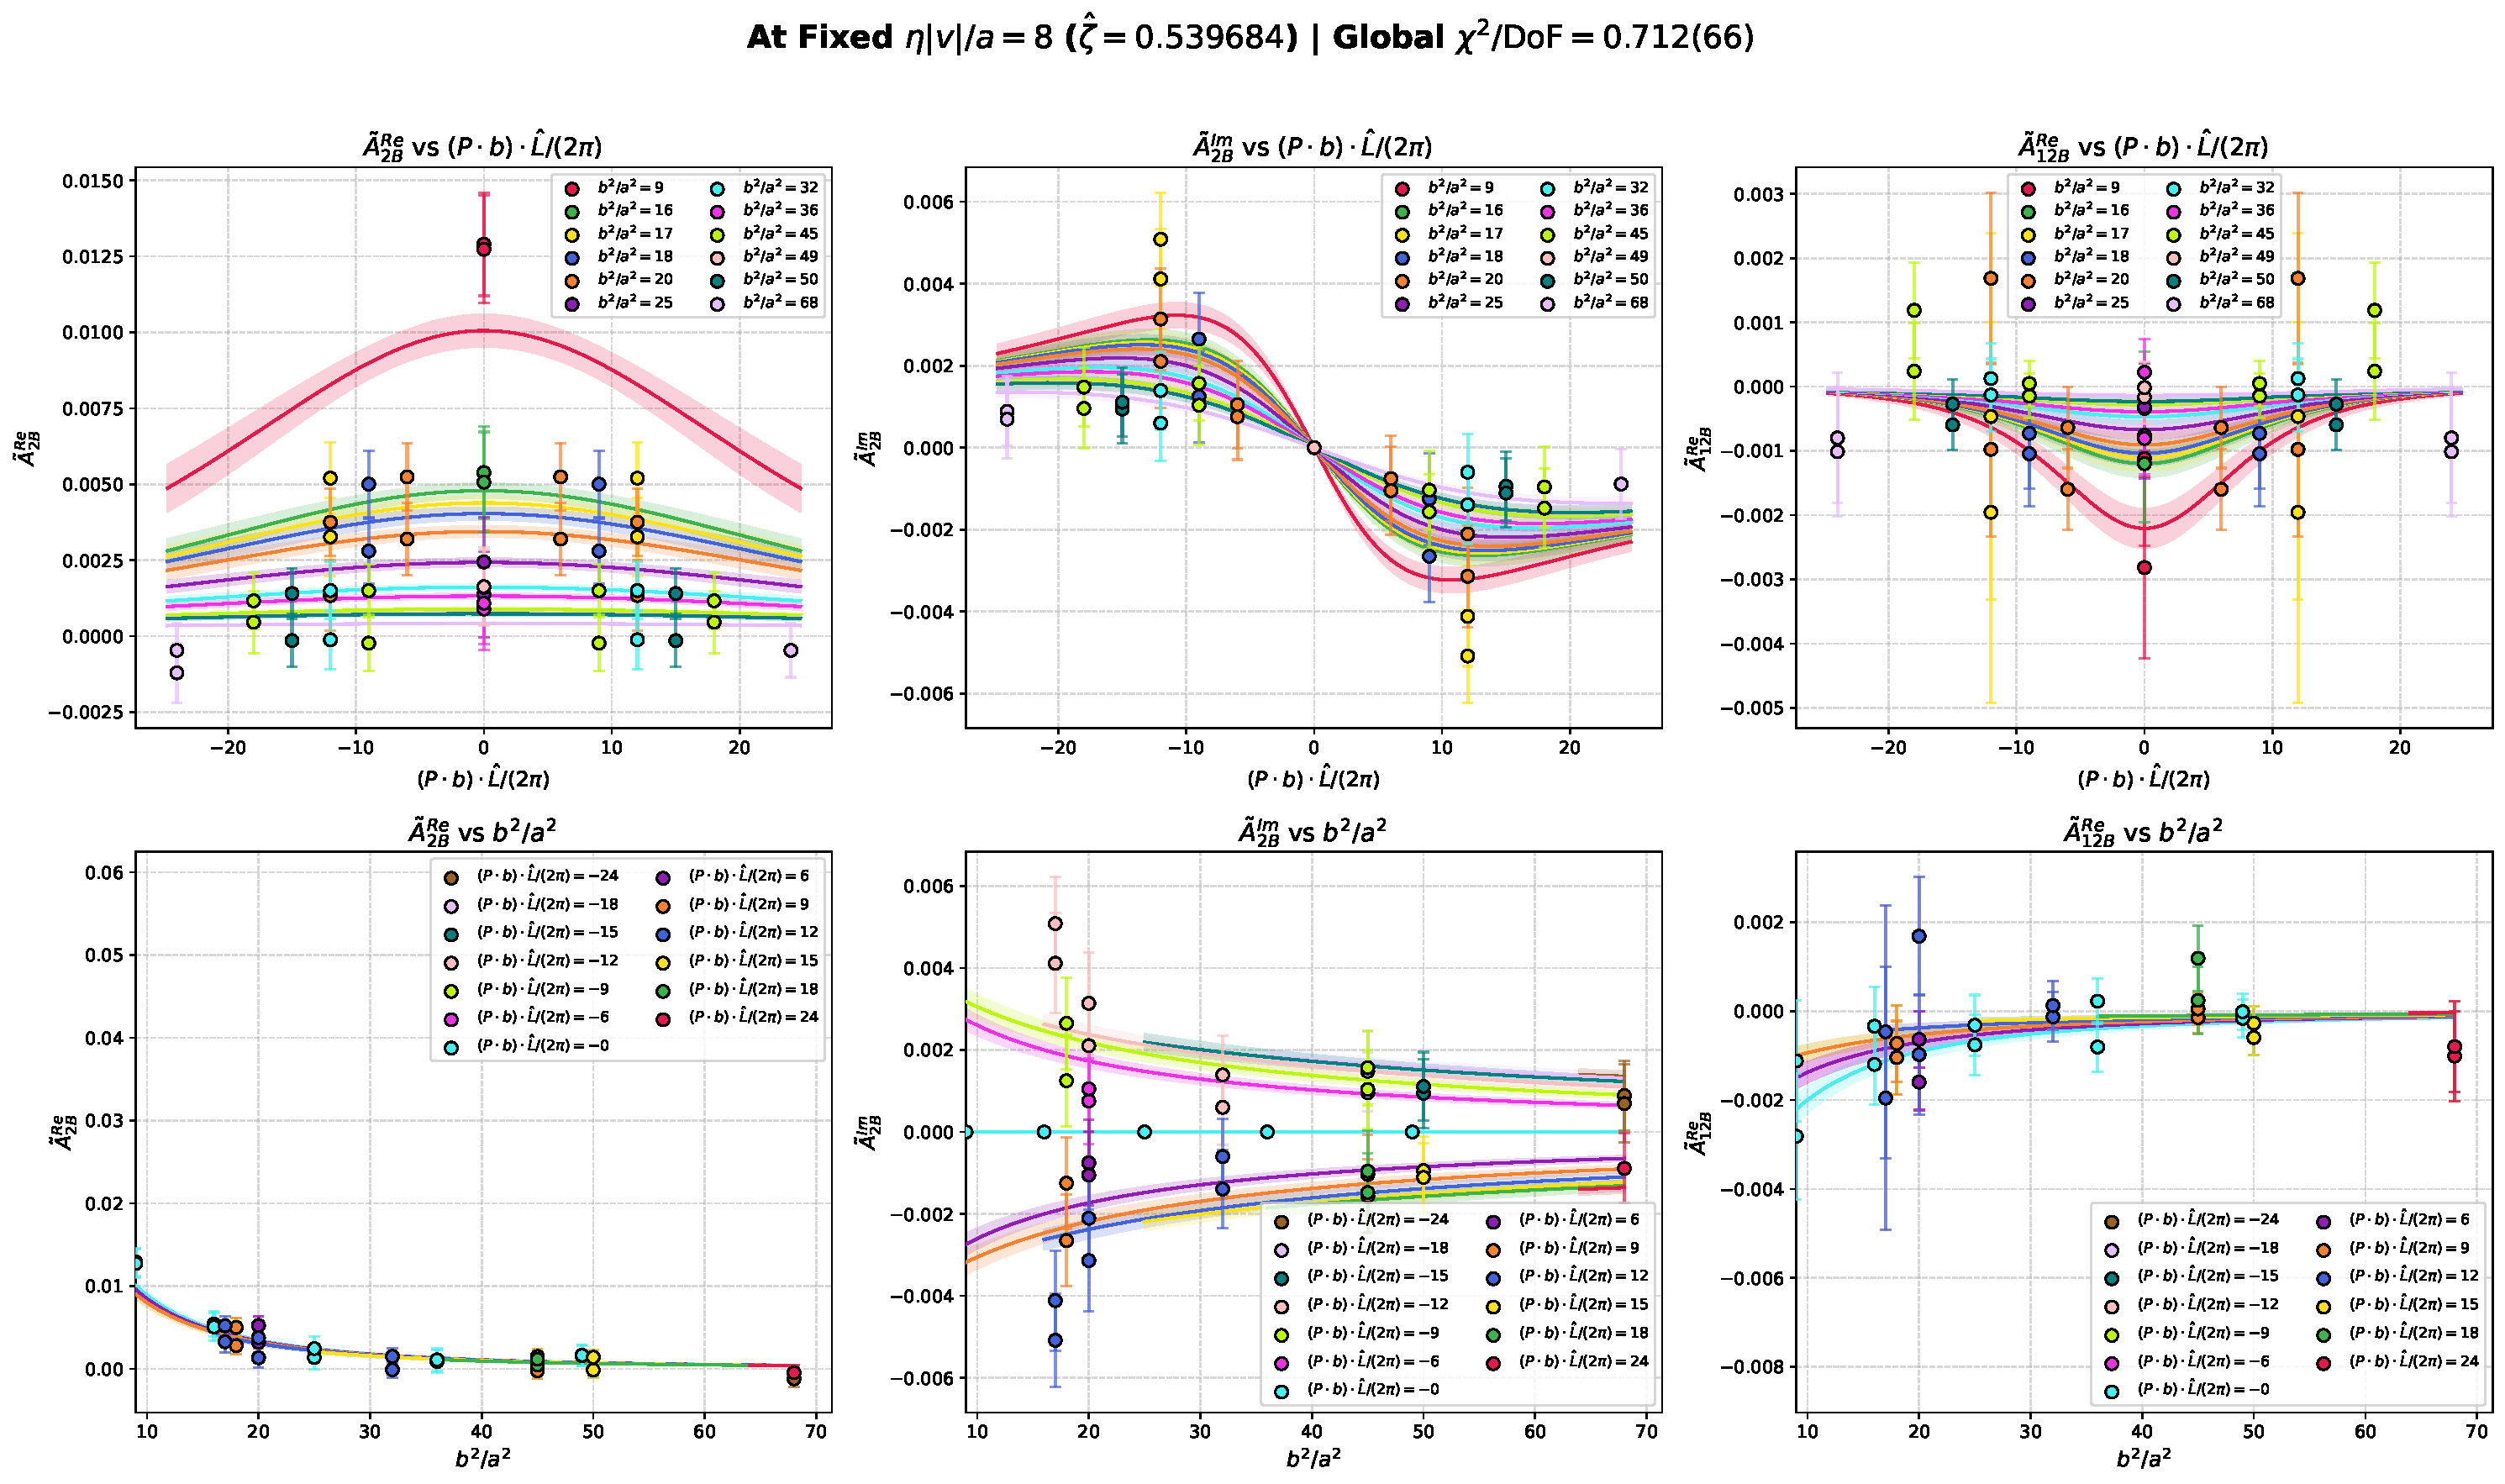
\includegraphics[height=0.82\textheight, keepaspectratio]{Combined_Pb_bsq_eta8_PL-3_WithFit_2D.pdf}
\end{frame}

% B12b
\begin{frame}{Backup: separable models vs the coupled power law}
  \centering
  {\scriptsize
  \renewcommand{\arraystretch}{1.3}\setlength{\tabcolsep}{3.5pt}
  \begin{tabular}{lccccccc}
    \toprule
    Model: longitudinal $\times$ transverse & \multicolumn{4}{c}{$\chi^2/\text{dof}$ at $P_L=-1,-2,-3,-4$} & $c^{\text{Im}}_{2B}$ & $c^{\text{Re}}_{12B}$ & $a^{\text{Im}}_{2B}$ \\
    \midrule
    $e^{-c|P\cdot b|}\times e^{-d|\vect b|}$ & $1.406(92)$ & $0.956(75)$ & $0.622(61)$ & $0.455(53)$ & $0.0010(262)$ & $0.045(23)$ & $-0.167(16)$ \\
    $e^{-c|P\cdot b|}\times(1+d\,b^2)^{-j}$ & $1.286(89)$ & $0.938(75)$ & $0.623(61)$ & $0.447(53)$ & $0.0045(248)$ & $0.028(24)$ & $-0.167(31)$ \\
    $e^{-c(P\cdot b)^2}\times e^{-d|\vect b|}$ & $2.389(121)$ & $2.005(111)$ & $0.945(76)$ & $0.453(52)$ & $0.568(171)$ & $0.0038(69)$ & $+0.050(121)$ \\
    $e^{-c(P\cdot b)^2}\times(1+d\,b^2)^{-j}$ & $2.316(120)$ & $1.981(111)$ & $0.948(76)$ & $0.448(52)$ & $0.602(48)$ & $0.0016(61)$ & $+0.168(92)$ \\
    \midrule
    \textbf{coupled power law in $(P\cdot b, b^2)$} & $1.85(10)$ & $1.197(85)$ & $0.712(66)$ & $0.434(51)$ & $\mathbf{0.2253(69)}$ & $\mathbf{0.0773(46)}$ & $\mathbf{+0.267(13)}$ \\
    \bottomrule
  \end{tabular}}
  \raggedright
  \begin{itemize}
    \item Parameters shown at $P_L=-1$. Separable models: $c^{\text{Im}}_{2B}$ or $c^{\text{Re}}_{12B}$ consistent with zero, $a^{\text{Im}}_{2B}$ sign flips, or poor $\chi^2$.
  \end{itemize}
\end{frame}

% B13a
\begin{frame}{Backup: ratio test directly on lattice data ($P_L=-1$)}
  \centering
  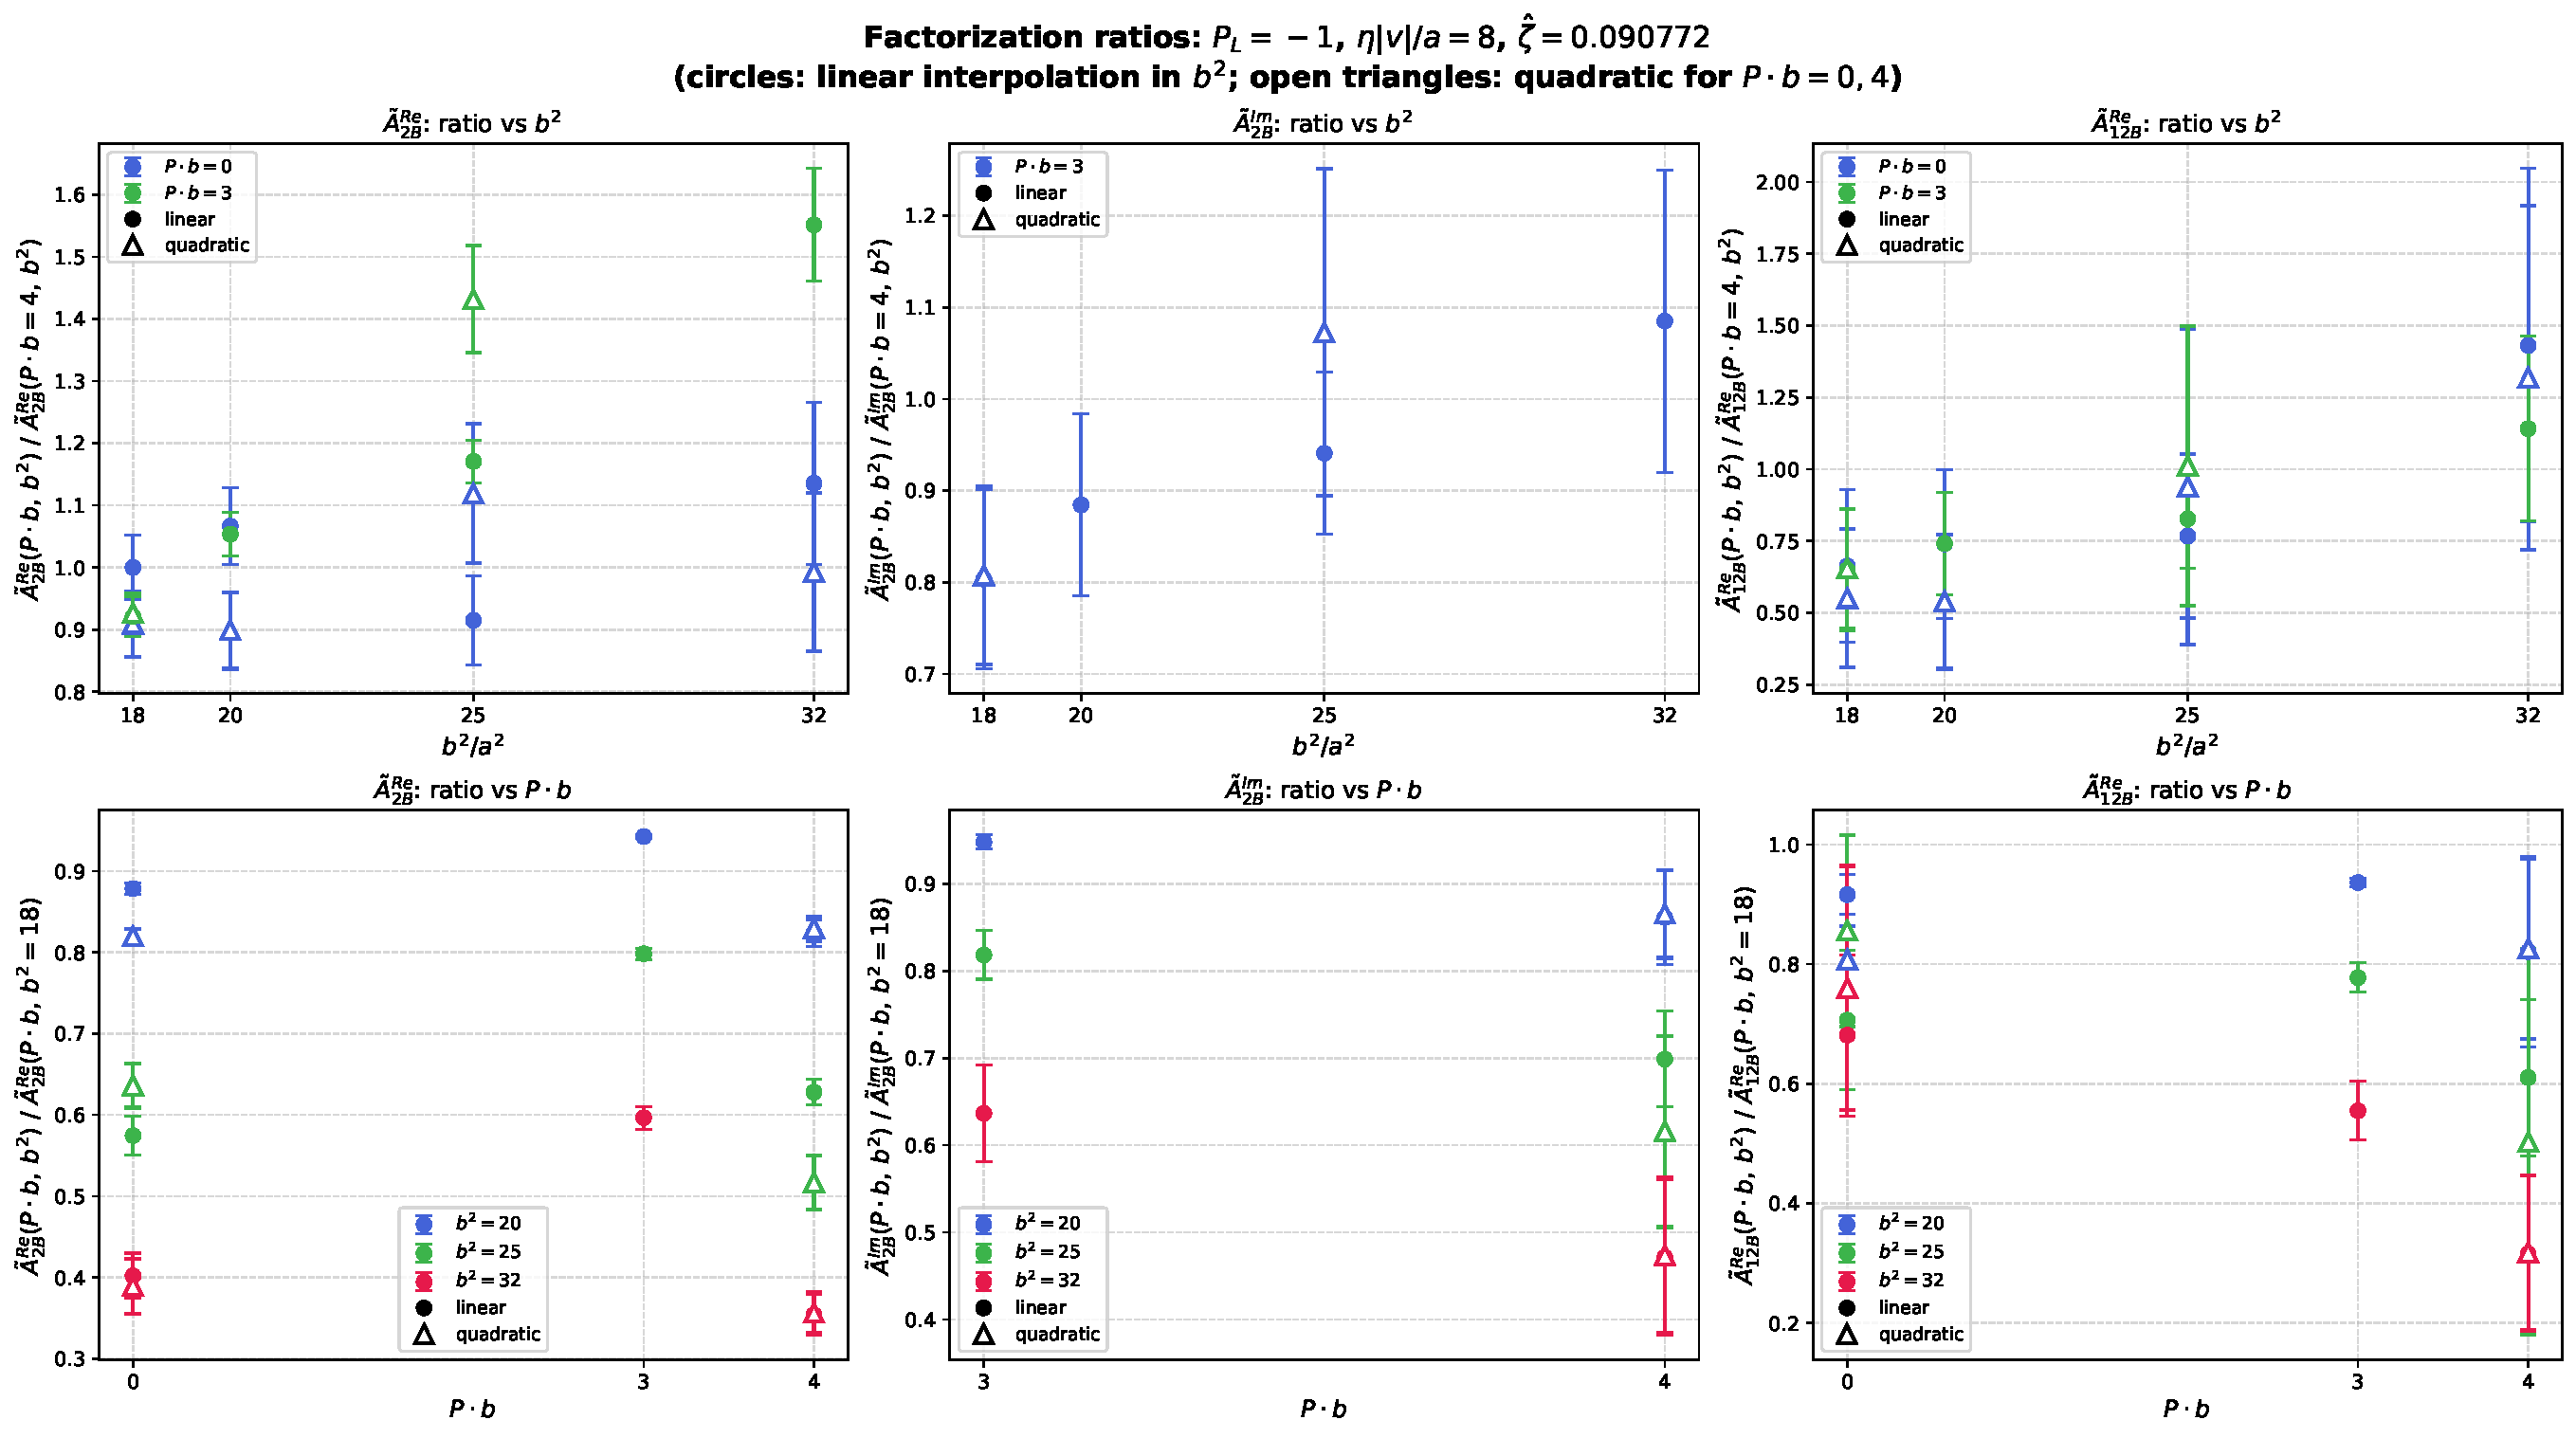
\includegraphics[height=0.82\textheight, keepaspectratio]{Factorization_ratios_Pb034_lin_vs_quad_eta8_PL-1.pdf}
\end{frame}

% B13b
\begin{frame}{Backup: optimal separable factors and reconstruction}
  \centering
  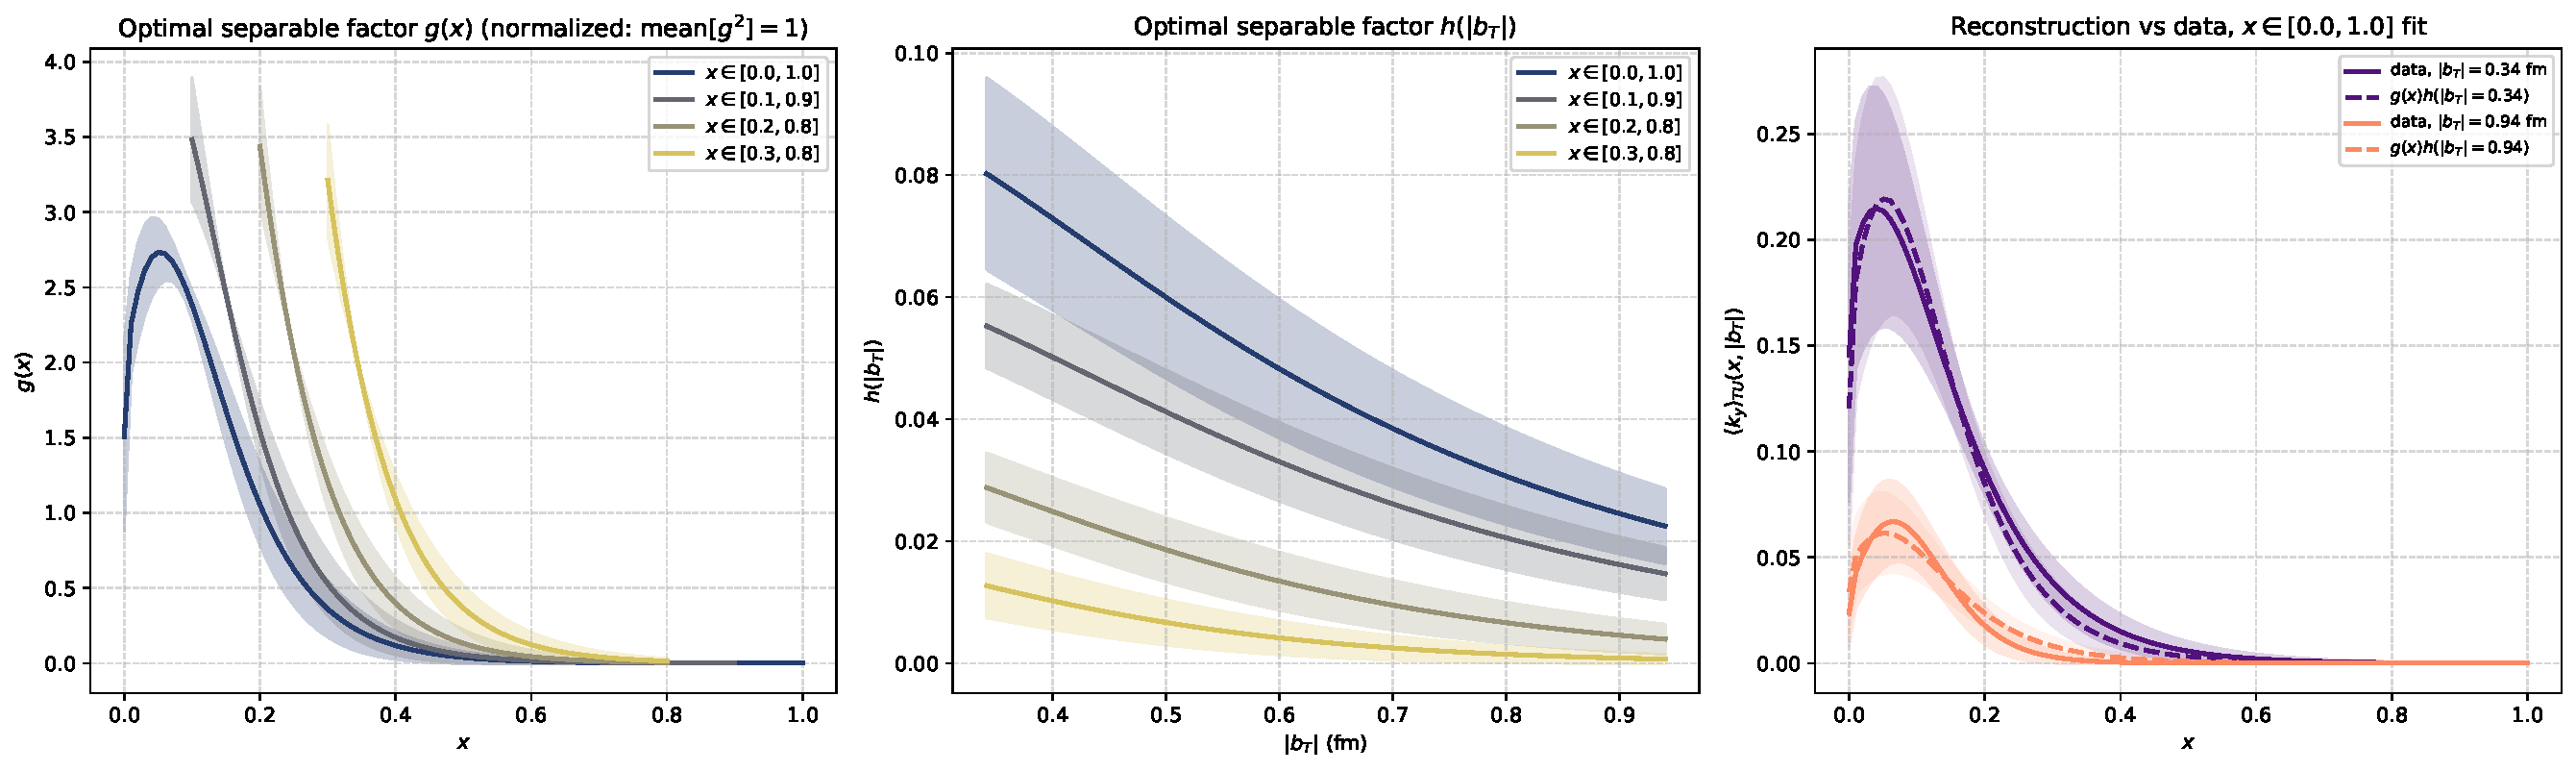
\includegraphics[width=\linewidth]{Factorization_gh_and_Reconstruction_bmin3_eta610.pdf}\\
  {\scriptsize Left: $g(x)$; middle: $h(|\vprp b|)$ for four $x$-windows; right: data vs $g(x)h(|\vprp b|)$ at $|\vprp b|=0.34$ and $0.94$ fm}
\end{frame}

% B14
\begin{frame}{Backup: soft factor and renormalization}
  \begin{itemize}
    \item At fixed geometry: under $\Gamma$-independent multiplicative renormalization, the soft factor and $Z$ cancel in $\tAmp_{12B}/\tAmp_{2B}$ at the same $(\bvec, P, \eta v)$.
    \item This work: ratios of amplitudes at fixed geometry, with $\bvec\tcdot P$ scanned and Fourier transformed.
    \item The $(-\infty,\infty)$ entry of the last row of the integral table equals the $\bvec\tcdot P=0$ ratio (an identity).
    % TODO(Hari): prepare the oral answer on what changes with b_L at fixed |b_T| (link length vs cusp angles)
  \end{itemize}
\end{frame}

% B15
\begin{frame}{Backup: generalized shifts of other TMDs}
  \small
  \begin{align*}
    \langle \vect{k}_y \rangle_{UT}(\vprp{\bvec}^2,x)
      &= \mN \frac{\int d(\bvec\tcdot P)\, e^{ix(\bvec\tcdot P)}\, \tAmp_{4B}}{\int d(\bvec\tcdot P)\, e^{ix(\bvec\tcdot P)}\, \tAmp_{2B}} & &\text{(Boer--Mulders, T-odd)} \\
    \langle \vect{k}_x \rangle_{TL}(\vprp{\bvec}^2,x)
      &= -\mN \frac{\int d(\bvec\tcdot P)\, e^{ix(\bvec\tcdot P)}\, \tAmp_{7B}}{\int d(\bvec\tcdot P)\, e^{ix(\bvec\tcdot P)}\, \tAmp_{2B}} & &\text{(worm-gear $g_{1T}$, T-even)} \\
    \frac{\tilde h_{1}^{(0)}}{\tilde f_1^{(0)}}(\vprp{\bvec}^2,x)
      &= -\frac{\int d(\bvec\tcdot P)\, e^{ix(\bvec\tcdot P)}\, \tAmp_{9Bm}}{\int d(\bvec\tcdot P)\, e^{ix(\bvec\tcdot P)}\, \tAmp_{2B}} & &\text{(tensor charge, T-even)}
  \end{align*}
  \normalsize
  \begin{itemize}
    \item Unlike the $x$-integrated shifts ($\bvec\tcdot P=0$ only), each needs a scan in $\bvec\tcdot P$ under the same kinematic constraint.
  \end{itemize}
\end{frame}
